%% The following is a directive for TeXShop to indicate the main file
%%!TEX root = diss.tex

\chapter{Introduction}
\label{ch:Introduction}

\begin{epigraph}
    \emph{If I have seen farther it is by standing on the shoulders of
    Giants.} ---~Sir Isaac Newton (1855)
\end{epigraph}

This document provides a quick set of instructions for using the
\class{ubcdiss} class to write a dissertation in \LaTeX. 
Unfortunately this document cannot provide an introduction to using
\LaTeX.  The classic reference for learning \LaTeX\ is
\citeauthor{lamport-1994-ladps}'s
book~\cite{lamport-1994-ladps}.  There are also many freely-available
tutorials online;
\webref{http://www.andy-roberts.net/misc/latex/}{Andy Roberts' online
    \LaTeX\ tutorials}
seems to be excellent.
The source code for this docment, however, is intended to serve as
an example for creating a \LaTeX\ version of your dissertation.

We start by discussing organizational issues, such as splitting
your dissertation into multiple files, in
\autoref{sec:SuggestedThesisOrganization}.
We then cover the ease of managing cross-references in \LaTeX\ in
\autoref{sec:CrossReferences}.
We cover managing and using bibliographies with \BibTeX\ in
\autoref{sec:BibTeX}. 
We briefly describe typesetting attractive tables in
\autoref{sec:TypesettingTables}.
We briefly describe including external figures in
\autoref{sec:Graphics}, and using special characters and symbols
in \autoref{sec:SpecialSymbols}.
As it is often useful to track different versions of your dissertation,
we discuss revision control further in
\autoref{sec:DissertationRevisionControl}. 
We conclude with pointers to additional sources of information in
\autoref{sec:Conclusions}.

%%%%%%%%%%%%%%%%%%%%%%%%%%%%%%%%%%%%%%%%%%%%%%%%%%%%%%%%%%%%%%%%%%%%%%
\section{Suggested Thesis Organization}
\label{sec:SuggestedThesisOrganization}

The \acs{UBC} \acf{GPS} specifies a particular arrangement of the
components forming a thesis.\footnote{See
    \url{http://www.grad.ubc.ca/current-students/dissertation-thesis-preparation/order-components}}
This template reflects that arrangement.

In terms of writing your thesis, the recommended best practice for
organizing large documents in \LaTeX\ is to place each chapter in
a separate file.  These chapters are then included from the main
file through the use of \verb+\include{file}+.  A thesis might
be described as six files such as \file{intro.tex},
\file{relwork.tex}, \file{model.tex}, \file{eval.tex},
\file{discuss.tex}, and \file{concl.tex}.

We also encourage you to use macros for separating how something
will be typeset (\eg bold, or italics) from the meaning of that
something. 
For example, if you look at \file{intro.tex}, you will see repeated
uses of a macro \verb+\file{}+ to indicate file names.
The \verb+\file{}+ macro is defined in the file \file{macros.tex}.
The consistent use of \verb+\file{}+ throughout the text not only
indicates that the argument to the macro represents a file (providing
meaning or semantics), but also allows easily changing how
file names are typeset simply by changing the definition of the
\verb+\file{}+ macro.
\file{macros.tex} contains other useful macros for properly typesetting
things like the proper uses of the latinate \emph{exempli grati\={a}}
and \emph{id est} (\ie \verb+\eg+ and \verb+\ie+), 
web references with a footnoted \acs{URL} (\verb+\webref{url}{text}+),
as well as definitions specific to this documentation
(\verb+\latexpackage{}+).

%%%%%%%%%%%%%%%%%%%%%%%%%%%%%%%%%%%%%%%%%%%%%%%%%%%%%%%%%%%%%%%%%%%%%%
\section{Making Cross-References}
\label{sec:CrossReferences}

\LaTeX\ make managing cross-references easy, and the \latexpackage{hyperref}
package's\ \verb+\autoref{}+ command\footnote{%
    The \latexpackage{hyperref} package is included by default in this
    template.}
makes it easier still. 

A thing to be cross-referenced, such as a section, figure, or equation,
is \emph{labelled} using a unique, user-provided identifier, defined
using the \verb+\label{}+ command.  
The thing is referenced elsewhere using the \verb+\autoref{}+ command.
For example, this section was defined using:
\begin{lstlisting}
    \section{Making Cross-References}
    \label{sec:CrossReferences}
\end{lstlisting}
References to this section are made as follows:
\begin{lstlisting}
    We then cover the ease of managing cross-references in \LaTeX\
    in \autoref{sec:CrossReferences}.
\end{lstlisting}
\verb+\autoref{}+ takes care of determining the \emph{type} of the 
thing being referenced, so the example above is rendered as
\begin{quote}
    We then cover the ease of managing cross-references in \LaTeX\
    in \autoref{sec:CrossReferences}.
\end{quote}

The label is any simple sequence of characters, numbers, digits,
and some punctuation marks such as ``:'' and ``--''; there should
be no spaces.  Try to use a consistent key format: this simplifies
remembering how to make references.  This document uses a prefix
to indicate the type of the thing being referenced, such as \texttt{sec}
for sections, \texttt{fig} for figures, \texttt{tbl} for tables,
and \texttt{eqn} for equations.

For details on defining the text used to describe the type
of \emph{thing}, search \file{diss.tex} and the \latexpackage{hyperref}
documentation for \texttt{autorefname}.


%%%%%%%%%%%%%%%%%%%%%%%%%%%%%%%%%%%%%%%%%%%%%%%%%%%%%%%%%%%%%%%%%%%%%%
\section{Managing Bibliographies with \BibTeX}
\label{sec:BibTeX}

One of the primary benefits of using \LaTeX\ is its companion program,
\BibTeX, for managing bibliographies and citations.  Managing
bibliographies has three parts: (i) describing references,
(ii)~citing references, and (iii)~formatting cited references.

\subsection{Describing References}

\BibTeX\ defines a standard format for recording details about a
reference.  These references are recorded in a file with a
\file{.bib} extension.  \BibTeX\ supports a broad range of
references, such as books, articles, items in a conference proceedings,
chapters, technical reports, manuals, dissertations, and unpublished
manuscripts. 
A reference may include attributes such as the authors,
the title, the page numbers, the \ac{DOI}, or a \ac{URL}.  A reference
can also be augmented with personal attributes, such as a rating,
notes, or keywords.

Each reference must be described by a unique \emph{key}.\footnote{%
    Note that the citation keys are different from the reference
    identifiers as described in \autoref{sec:CrossReferences}.}
A key is a simple sequence of characters, numbers, digits, and some
punctuation marks such as ``:'' and ``--''; there should be no spaces. 
A consistent key format simiplifies remembering how to make references. 
For example:
\begin{quote}
   \fbox{\emph{last-name}}\texttt{-}\fbox{\emph{year}}\texttt{-}\fbox{\emph{contracted-title}}
\end{quote}
where \emph{last-name} represents the last name for the first author,
and \emph{contracted-title} is some meaningful contraction of the
title.  Then \citeauthor{kiczales-1997-aop}'s seminal article on
aspect-oriented programming~\cite{kiczales-1997-aop} (published in
\citeyear{kiczales-1997-aop}) might be given the key
\texttt{kiczales-1997-aop}.

An example of a \BibTeX\ \file{.bib} file is included as
\file{biblio.bib}.  A description of the format a \file{.bib}
file is beyond the scope of this document.  We instead encourage
you to use one of the several reference managers that support the
\BibTeX\ format such as
\webref{http://jabref.sourceforge.net}{JabRef} (multiple platforms) or
\webref{http://bibdesk.sourceforge.net}{BibDesk} (MacOS\,X only). 
These front ends are similar to reference manages such as
EndNote or RefWorks.


\subsection{Citing References}

Having described some references, we then need to cite them.  We
do this using a form of the \verb+\cite+ command.  For example:
\begin{lstlisting}
    \citet{kiczales-1997-aop} present examples of crosscutting 
    from programs written in several languages.
\end{lstlisting}
When processed, the \verb+\citet+ will cause the paper's authors
and a standardized reference to the paper to be inserted in the
document, and will also include a formatted citation for the paper
in the bibliography.  For example:
\begin{quote}
    \citet{kiczales-1997-aop} present examples of crosscutting 
    from programs written in several languages.
\end{quote}
There are several forms of the \verb+\cite+ command (provided
by the \latexpackage{natbib} package), as demonstrated in
\autoref{tbl:natbib:cite}.
Note that the form of the citation (numeric or author-year) depends
on the bibliography style (described in the next section).
The \verb+\citet+ variant is used when the author names form
an object in the sentence, whereas the \verb+\citep+ variant
is used for parenthetic references, more like an end-note.
\begin{table}
\caption{Available \texttt{cite} variants; the exact citation style
    depends on whether the bibliography style is numeric or author-year.}
\label{tbl:natbib:cite}
\centering
\begin{tabular}{lp{3.25in}}\toprule
Variant & Result \\
\midrule
% We cheat here to simulate the cite/citep/citet for APA-like styles
\verb+\cite+ & Parenthetical citation (\eg ``\cite{kiczales-1997-aop}''
    or ``(\citeauthor{kiczales-1997-aop} \citeyear{kiczales-1997-aop})'') \\
\verb+\citet+ & Textual citation: includes author (\eg
    ``\citet{kiczales-1997-aop}'' or
    or ``\citeauthor{kiczales-1997-aop} (\citeyear{kiczales-1997-aop})'') \\
\verb+\citet*+ & Textual citation with unabbreviated author list \\
\verb+\citealt+ & Like \verb+\citet+ but without parentheses \\
\verb+\citep+ & Parenthetical citation (\eg ``\cite{kiczales-1997-aop}''
    or ``(\citeauthor{kiczales-1997-aop} \citeyear{kiczales-1997-aop})'') \\
\verb+\citep*+ & Parenthetical citation with unabbreviated author list \\
\verb+\citealp+ & Like \verb+\citep+ but without parentheses \\
\verb+\citeauthor+ & Author only (\eg ``\citeauthor{kiczales-1997-aop}'') \\
\verb+\citeauthor*+ & Unabbreviated authors list 
    (\eg ``\citeauthor*{kiczales-1997-aop}'') \\
\verb+\citeyear+ & Year of citation (\eg ``\citeyear{kiczales-1997-aop}'') \\
\bottomrule
\end{tabular}
\end{table}

\subsection{Formatting Cited References}

\BibTeX\ separates the citing of a reference from how the cited
reference is formatted for a bibliography, specified with the
\verb+\bibliographystyle+ command. 
There are many varieties, such as \texttt{plainnat}, \texttt{abbrvnat},
\texttt{unsrtnat}, and \texttt{vancouver}.
This document was formatted with \texttt{abbrvnat}.
Look through your \TeX\ distribution for \file{.bst} files. 
Note that use of some \file{.bst} files do not emit all the information
necessary to properly use \verb+\citet{}+, \verb+\citep{}+,
\verb+\citeyear{}+, and \verb+\citeauthor{}+.

There are also packages available to place citations on a per-chapter
basis (\latexpackage{bibunits}), as footnotes (\latexpackage{footbib}),
and inline (\latexpackage{bibentry}).
Those who wish to exert maximum control over their bibliography
style should see the amazing \latexpackage{custom-bib} package.

%%%%%%%%%%%%%%%%%%%%%%%%%%%%%%%%%%%%%%%%%%%%%%%%%%%%%%%%%%%%%%%%%%%%%%
\section{Typesetting Tables}
\label{sec:TypesettingTables}

\citet{lamport-1994-ladps} made one grievous mistake
in \LaTeX: his suggested manner for typesetting tables produces
typographic abominations.  These suggestions have unfortunately
been replicated in most \LaTeX\ tutorials.  These
abominations are easily avoided simply by ignoring his examples
illustrating the use of horizontal and vertical rules (specifically
the use of \verb+\hline+ and \verb+|+) and using the
\latexpackage{booktabs} package instead.

The \latexpackage{booktabs} package helps produce tables in the form
used by most professionally-edited journals through the use of
three new types of dividing lines, or \emph{rules}.
% There are times that you don't want to use \autoref{}
Tables~\ref{tbl:natbib:cite} and~\ref{tbl:LaTeX:Symbols} are two
examples of tables typeset with the \latexpackage{booktabs} package.
The \latexpackage{booktabs} package provides three new commands
for producing rules:
\verb+\toprule+ for the rule to appear at the top of the table,
\verb+\midrule+ for the middle rule following the table header,
and \verb+\bottomrule+ for the bottom-most at the end of the table.
These rules differ by their weight (thickness) and the spacing before
and after.
A table is typeset in the following manner:
\begin{lstlisting}
    \begin{table}
    \caption{The caption for the table}
    \label{tbl:label}
    \centering
    \begin{tabular}{cc}
    \toprule
    Header & Elements \\
    \midrule
    Row 1 & Row 1 \\
    Row 2 & Row 2 \\
    % ... and on and on ...
    Row N & Row N \\
    \bottomrule
    \end{tabular}
    \end{table}
\end{lstlisting}
See the \latexpackage{booktabs} documentation for advice in dealing with
special cases, such as subheading rules, introducing extra space
for divisions, and interior rules.

%%%%%%%%%%%%%%%%%%%%%%%%%%%%%%%%%%%%%%%%%%%%%%%%%%%%%%%%%%%%%%%%%%%%%%
\section{Figures, Graphics, and Special Characters}
\label{sec:Graphics}

Most \LaTeX\ beginners find figures to be one of the more challenging
topics.  In \LaTeX, a figure is a \emph{floating element}, to be
placed where it best fits.
The user is not expected to concern him/herself with the placement
of the figure.  The figure should instead be labelled, and where
the figure is used, the text should use \verb+\autoref+ to reference
the figure's label.
\autoref{fig:latex-affirmation} is an example of a figure.
\begin{figure}
    \centering
    % For the sake of this example, we'll just use text
    %\includegraphics[width=3in]{file}
    \Huge{\textsf{\LaTeX\ Rocks!}}
    \caption{Proof of \LaTeX's amazing abilities}
    \label{fig:latex-affirmation}   % label should change
\end{figure}
A figure is generally included as follows:
\begin{lstlisting}
    \begin{figure}
    \centering
    \includegraphics[width=3in]{file}
    \caption{A useful caption}
    \label{fig:fig-label}   % label should change
    \end{figure}
\end{lstlisting}
There are three items of note:
\begin{enumerate}
\item External files are included using the \verb+\includegraphics+
    command.  This command is defined by the \latexpackage{graphicx} package
    and can often natively import graphics from a variety of formats.
    The set of formats supported depends on your \TeX\ command processor.
    Both \texttt{pdflatex} and \texttt{xelatex}, for example, can
    import \textsc{gif}, \textsc{jpg}, and \textsc{pdf}.  The plain
    version of \texttt{latex} only supports \textsc{eps} files.

\item The \verb+\caption+ provides a caption to the figure. 
    This caption is normally listed in the List of Figures; you
    can provide an alternative caption for the LoF by providing
    an optional argument to the \verb+\caption+ like so:
    \begin{lstlisting}
    \caption[nice shortened caption for LoF]{%
	longer detailed caption used for the figure}
    \end{lstlisting}
    \ac{GPS} generally prefers shortened single-line captions
    in the LoF: multiple-line captions are a bit unwieldy.

\item The \verb+\label+ command provides for associating a unique, user-defined,
    and descriptive identifier to the figure.  The figure can be
    can be referenced elsewhere in the text with this identifier
    as described in \autoref{sec:CrossReferences}.
\end{enumerate}
See Keith Reckdahl’s excellent guide for more details,
\webref{http://www.ctan.org/tex-archive/info/epslatex.pdf}{\emph{Using
imported graphics in LaTeX2e}}.

\section{Special Characters and Symbols}
\label{sec:SpecialSymbols}

\LaTeX\ appropriates many common symbols for its own purposes,
with some used for commands (\ie \verb+\{}&%+) and
mathematics (\ie \verb+$^_+), and others are automagically transformed
into typographically-preferred forms (\ie \verb+-`'+) or to
completely different forms (\ie \verb+<>+).
\autoref{tbl:LaTeX:Symbols} presents a list of common symbols and
their corresponding \LaTeX\ commands.  A much more comprehensive list 
of symbols and accented characters is available at:
\url{http://www.ctan.org/tex-archive/info/symbols/comprehensive/}
\begin{table}
\caption{Useful \LaTeX\ symbols}\label{tbl:LaTeX:Symbols}
\centering\begin{tabular}{ccp{0.5cm}cc}\toprule
\LaTeX & Result && \LaTeX & Result \\
\midrule
    \verb+\texttrademark+ & \texttrademark && \verb+\&+ & \& \\
    \verb+\textcopyright+ & \textcopyright && \verb+\{ \}+ & \{ \} \\
    \verb+\textregistered+ & \textregistered && \verb+\%+ & \% \\
    \verb+\textsection+ & \textsection && \verb+\verb!~!+ & \verb!~! \\
    \verb+\textdagger+ & \textdagger && \verb+\$+ & \$ \\
    \verb+\textdaggerdbl+ & \textdaggerdbl && \verb+\^{}+ & \^{} \\
    \verb+\textless+ & \textless && \verb+\_+ & \_ \\
    \verb+\textgreater+ & \textgreater && \\
\bottomrule
\end{tabular}
\end{table}

%%%%%%%%%%%%%%%%%%%%%%%%%%%%%%%%%%%%%%%%%%%%%%%%%%%%%%%%%%%%%%%%%%%%%%
\section{Changing Page Widths and Heights}

The \class{ubcdiss} class is based on the standard \LaTeX\ \class{book}
class that selects a line-width to carry approximately 66~characters
per line.  This character density is claimed to have a pleasing
appearance and also supports more rapid
reading~\cite{bringhurst-2002-teots}.  I would recommend that you
not change the line-widths!

\subsection{The \texttt{geometry} Package}

Some students are unfortunately saddled with misguided supervisors
or committee members whom believe that documents should have the
narrowest margins possible.  The \latexpackage{geometry} package is
helpful in such cases.  Using this package is as simple as:
\begin{lstlisting}
    \usepackage[margin=1.25in,top=1.25in,bottom=1.25in]{geometry}
\end{lstlisting}
You should check the package's documentation for more complex uses.

\subsection{Changing Page Layout Values By Hand}

There are some miserable students with requirements for page layouts
that vary throughout the document.  Unfortunately the
\latexpackage{geometry} can only be specified once, in the document's
preamble.  Such miserable students must set \LaTeX's layout parameters
by hand:
\begin{lstlisting}
    \setlength{\topmargin}{-.75in}
    \setlength{\headsep}{0.25in}
    \setlength{\headheight}{15pt}
    \setlength{\textheight}{9in}
    \setlength{\footskip}{0.25in}
    \setlength{\footheight}{15pt}

    % The *sidemargin values are relative to 1in; so the following
    % results in a 0.75 inch margin
    \setlength{\oddsidemargin}{-0.25in}
    \setlength{\evensidemargin}{-0.25in}
    \setlength{\textwidth}{7in}       % 1.1in margins (8.5-2*0.75)
\end{lstlisting}
These settings necessarily require assuming a particular page height
and width; in the above, the setting for \verb+\textwidth+ assumes
a \textsc{US} Letter with an 8.5'' width.
The \latexpackage{geometry} package simply uses the page height and
other specified values to derive the other layout values.
The
\href{http://tug.ctan.org/tex-archive/macros/latex/required/tools/layout.pdf}{\texttt{layout}}
package provides a
handy \verb+\layout+ command to show the current page layout
parameters. 


\subsection{Making Temporary Changes to Page Layout}

There are occasions where it becomes necessary to make temporary
changes to the page width, such as to accomodate a larger formula. 
The \latexmiscpackage{chngpage} package provides an \env{adjustwidth}
environment that does just this.  For example:
\begin{lstlisting}
    % Expand left and right margins by 0.75in
    \begin{adjustwidth}{-0.75in}{-0.75in}
    % Must adjust the perceived column width for LaTeX to get with it.
    \addtolength{\columnwidth}{1.5in}
    \[ an extra long math formula \]
    \end{adjustwidth}
\end{lstlisting}


%%%%%%%%%%%%%%%%%%%%%%%%%%%%%%%%%%%%%%%%%%%%%%%%%%%%%%%%%%%%%%%%%%%%%%
\section{Keeping Track of Versions with Revision Control}
\label{sec:DissertationRevisionControl}

Software engineers have used \acf{RCS} to track changes to their
software systems for decades.  These systems record the changes to
the source code along with context as to why the change was required.
These systems also support examining and reverting to particular
revisions from their system's past.

An \ac{RCS} can be used to keep track of changes to things other
than source code, such as your dissertation.  For example, it can
be useful to know exactly which revision of your dissertation was
sent to a particular committee member.  Or to recover an accidentally
deleted file, or a badly modified image.  With a revision control
system, you can tag or annotate the revision of your dissertation
that was sent to your committee, or when you incorporated changes
from your supervisor.

Unfortunately current revision control packages are not yet targetted
to non-developers.  But the Subversion project's
\webref{http://tortoisesvn.net/docs/release/TortoiseSVN_en/}{TortoiseSVN}
has greatly simplified using the Subversion revision control system
for Windows users.  You should consult your local geek.

A simpler alternative strategy is to create a GoogleMail account
and periodically mail yourself zipped copies of your dissertation.

%%%%%%%%%%%%%%%%%%%%%%%%%%%%%%%%%%%%%%%%%%%%%%%%%%%%%%%%%%%%%%%%%%%%%%
\section{Recommended Packages}

The real strength to \LaTeX\ is found in the myriad of free add-on
packages available for handling special formatting requirements.
In this section we list some helpful packages.

\subsection{Typesetting}

\begin{description}
\item[\latexpackage{enumitem}:]
    Supports pausing and resuming enumerate environments.

\item[\latexpackage{ulem}:]
    Provides two new commands for striking out and crossing out text
    (\verb+\sout{text}+ and \verb+\xout{text}+ respectively)
    The package should likely
    be used as follows:
    \begin{verbatim}
    \usepackage[normalem,normalbf]{ulem}
    \end{verbatim}
    to prevent the package from redefining the emphasis and bold fonts.

\item[\latexpackage{chngpage}:]
    Support changing the page widths on demand.

\item[\latexpackage{mhchem}:] 
    Support for typesetting chemical formulae and reaction equations.

\end{description}

Although not a package, the
\webref{http://www.ctan.org/tex-archive/support/latexdiff/}{\texttt{latexdiff}}
command is very useful for creating changebar'd versions of your
dissertation.


\subsection{Figures, Tables, and Document Extracts}

\begin{description}
\item[\latexpackage{pdfpages}:]
    Insert pages from other PDF files.  Allows referencing the extracted
    pages in the list of figures, adding labels to reference the page
    from elsewhere, and add borders to the pages.

\item[\latexpackage{subfig}:]
    Provides for including subfigures within a figure, and includes
    being able to separately reference the subfigures.  This is a
    replacement for the older \texttt{subfigure} environment.

\item[\latexpackage{rotating}:]
    Provides two environments, sidewaystable and sidewaysfigure,
    for typesetting tables and figures in landscape mode.  

\item[\latexpackage{longtable}:]
    Support for long tables that span multiple pages.

\item[\latexpackage{tabularx}:]
    Provides an enhanced tabular environment with auto-sizing columns.

\item[\latexpackage{ragged2e}:]
    Provides several new commands for setting ragged text (\eg forms
    of centered or flushed text) that can be used in tabular
    environments and that support hyphenation.

\end{description}


\subsection{Bibliography Related Packages}

\begin{description}
\item[\latexpackage{bibunits}:]
    Support having per-chapter bibliographies.

\item[\latexpackage{footbib}:]
    Cause cited works to be rendered using footnotes.

\item[\latexpackage{bibentry}:] 
    Support placing the details of a cited work in-line.

\item[\latexpackage{custom-bib}:]
    Generate a custom style for your bibliography.

\end{description}


%%%%%%%%%%%%%%%%%%%%%%%%%%%%%%%%%%%%%%%%%%%%%%%%%%%%%%%%%%%%%%%%%%%%%%
\section{Moving On}
\label{sec:Conclusions}

At this point, you should be ready to go.  Other handy web resources:
\begin{itemize}
\item \webref{http://www.ctan.org}{\ac{CTAN}} is \emph{the} comprehensive
    archive site for all things related to \TeX\ and \LaTeX. 
    Should you have some particular requirement, somebody else is
    almost certainly to have had the same requirement before you,
    and the solution will be found on \ac{CTAN}.  The links to
    various packages in this document are all to \ac{CTAN}.

\item An online
    \webref{http://www.ctan.org/get/info/latex2e-help-texinfo/latex2e.html}{%
	reference to \LaTeX\ commands} provides a handy quick-reference
    to the standard \LaTeX\ commands.

\item The list of 
    \webref{http://www.tex.ac.uk/cgi-bin/texfaq2html?label=interruptlist}{%
	Frequently Asked Questions about \TeX\ and \LaTeX}
    can save you a huge amount of time in finding solutions to
    common problems.

\item The \webref{http://www.tug.org/tetex/tetex-texmfdist/doc/}{te\TeX\
    documentation guide} features a very handy list of the most useful
    packages for \LaTeX\ as found in \ac{CTAN}.

\item The
\webref{http://www.ctan.org/tex-archive/macros/latex/required/graphics/grfguide.pdf}{\texttt{color}}
    package, part of the graphics bundle, provides handy commands
    for changing text and background colours.  Simply changing
    text to various levels of grey can have a very 
    \textcolor{greytext}{dramatic effect}.


\item If you're really keen, you might want to join the
    \webref{http://www.tug.org}{\TeX\ Users Group}.

\end{itemize}

%=======================================
\section{Brief Note on Notation}
\label{sec:Brief}
%=======================================

We'll investigate the generating functions for quarter-plane walks where we track how many times these walks touch the walls. 
\begin{itemize}
\item $Q$ is the generating function.
\item Powers of variables $x_i$ keep track of the $i$-th coordinate of the endpoint of a random walk. For example the monomial $x_1^3x_2^1x_4^7$ counts how many walks end at $(3,1,0,7)$.
\item Powers of variables $a_i$ keep track of the number of times a random walk passes through a point with $i$-th coordinate equal to zero. For example the monomial $a_1^2a_2$ counts how many times the random walks have passed through points with coordinates $(0,j)$ and $(i,0)$ respectively.
\item Powers of $t$ count the length of random walks.
\item Variables with overline are reciprocals like $\ol{x_1} = 1/x_1$.
\item $S$ is the Laurent polynomial generating function for the allowed step set. For example for the steps $\{$N, E, SW$\}$ we have $S = x_2 + x_1+\ol{x_1}\ol{x_2}$.
\item We'll often use $b_i = a_1-1$ and $c_i = b_i/a_i = 1-\ol{a_i}$.
\end{itemize}
Next we have some notation on extraction of coefficients
\begin{itemize}
\item $[d] = (1,\ldots,d)$ as a sequence.
\item For a sequence $I = (i_1,\ldots, i_n)$ and a sequence $P = (p_1,\ldots,p_n)$, $x_I^P = x_{i_1}^{p_1}\ldots x_{i_n}^{p_n}$. For example $x_{[3]}^{(1,0,2)} = x_1^1x_2^0x_3^2 = x_1x_3^2$. We'll usually use this notation for when we have general sequences, not in the case of the example which we would write out explicitly.
\item $[u_I^P]$ stands for extracting the coefficient infront of $u_I^P$ in the generating function expansion.
\item $Q_{I}^J = [x_I^P]Q$ and similarly $S_I^J =[x_I^J]S$. For example if $I = (1,3)$, $J = {0,1}$, (omiting parentheses) $Q_I^J = Q_{1,3}^{0,1}$. We will sometimes write $(Q_I^P)_J^R = Q_{I,J}^{P,R}$
\item For a set $I$, $\oo$ and $\one$ stand for sequences of $|I|$ zeros and ones respectively. For example for $I \subseteq [d]$ we might have $S_I^{-\one}Q_I^{\oo}$. Analogously we will write $(Q_I^{\one})_J^\oo = Q_{I,J}^{\one,\oo}$
\end{itemize}
So we have
\[
	Q(x_1,x_2,a_1,a_2;t) = \sum_{i,j,k} \Qf{i,j}x_1^i x_2^j t^k
\]
So far we won't extract $a$'s because we have an unobvious choice between extracting $a,b$ or $c$ with various pros/cons. For example it may sometimes be easier to extract $b_1^k$ than $a_1^k$ but there's the added cost that the extracted term counts walks with varying powers of $k$. We usually won't extract with respect to $t$.

%=======================================
\section{Introduction to Methods - 1D random walks}
%=======================================
%=======================================
\subsection{Derivation of the functional equation}
%=======================================

In the interest of working out higher dimensional labelled walks' problems it is very useful to first visit the 1-dimensional case which will illustrate a lot of the methods that will later come into play. The 1-dimensional case will also give us a clearer picture as to how things work in higher dimensions (although the picture becomes more complicated). We'll treat the problem using generating functions. We'll use lower case letters and not quite the full notation because it is not necessary. In one dimension, on one axis, we'll use steps of length at most 1. If we have a random walk ending at coordinate $i$ we can either step back adding $-1$ to the coordinate, step forward adding $+1$ to the coordinate or staying in one place, adding $0$ to the coordinate. This can be somewhat formalized by using polynomials. Ending a walk at coordinate $i$ will be encoded with a monomial $x^i$. Then stepping backwards, forwards or staying in one place will be denoted with $x^{i-1}$, $x^i$ and $x^{i+1}$ respectively. This is the same as multiplying by $1/x = \ol{x}, 1, x$ in each case. We can encode this information is a Laurent step polynomial $s$ defined as
\[
	s = s_{-1}\ol{x} + s_0 + s_1 x
\]
Here $s_i$ will be either 0 or 1 for any specific $i$, tracking whether we have allowed those kinds of steps or not. Keeping this in mind, there are 8 possible step sets because we have two options for each $s_i$. We keep track of the length of a random walk with powers of $t$ and we keep track of its endpoint with powers of $x$. We'll also label every interaction with the origin by multiplying by $a$ every time a walk steps on the origin. We'll keep the walks on the non-negative axis.

Long story short we can find the generating function in a very simple, brute force manner, even for higher dimensions. We start with the empty walk denoted by 1 since it starts and ends on the origin without taking a step, so no $t$, $x$ or label $a$. Then try out each step from $s$ and eliminate those that take us past the origin in the negative direction. If we step on the origin we multiply by $a$. Those walks that remain are then multiplied by $t$ since they are not of length 1. We can proceed iteratively $k$ tiems to obtain random walks on the non-negative axis of length $k$. Adding up the results allows us to write the generating function up to $O(t^k)$. It will prove very useful to think about operators so we can formalize this notion in terms of operators. For example, here we are taking walks of length $k-1$, trying all options of $s$ (this is like multiplying by $s$), removing all the walks that end up on the negative axis (this is like removing the $\ol{x}$ term) and labeling those that end on the origin (this is like multiplying the $x^0$ coefficient by $a$). Let $D$ stand for the operator that cleans up the walks and labels the valid ones. Then if $q_k$ stands for the labelled walks of length $k$, then the $k$-th term of $q$ is $q_k t^k$ and we have
\[
	q_{k+1}t^{k+1} = t D (s q_k t^k)
\]
Thus we can write the generating function $q$ iteratively
\[
	q = \sum_{k=0}^\infty t^k(Ds)^k(1)
\]
where we're iteratively applying $Ds$ to 1 to obtain all labelled walks. We can treat this operator $Ds$ as a formal variable and write
\[
	q = \sum_{k=0}^\infty (tDs)^k(1) = \frac{1}{1-tDs}(1)
\]
and then this gives us a functional equation for $q$
\[
	(1-tDs)q  =1 
\]
There is another way of deriving this equation while not treating $Ds$ as a formal variable. Instead of applying the operator iteratively we can apply it on the generating function as a whole. The product $tsq$ is the generating for all random walks that end with $x$-coordinate greater or equal to $-1$ where some steps end up on $x$-coordinate 0 without being labelled. We can apply $D$ on this product to remove the terms ending at $x$-coordinate $-1$ and label those that end up on $x$-coordinate 0. This leaves us with all the valid walks encoded in the generating function $q$ without the empty walk 1. Therefore we can write a functional equation for $q$ as
\[
	q = 1 + D(tsq) = 1 + tDs(q)
\]
and we ca re-write this as $(1-tDs)q  =1$ as before. Now, we have to say a few words about what the operator $D$ actually is. First we are removing all the walks that end on $x$-coordinate equal to $-1$ which can be handled by the operator $E = 1 - \ol{x}[\ol{x}]$ which removes those walks. Then the labelling can be handled by the operator $L = 1 + (a-1) [x^0] = 1 + b[x^0]$ where $b = a-1$. Therefore we can write $D  = LE$
\begin{align*}
	D &= LE = (1 - \ol{x}[\ol{x}])(1 + b[x^0]) \\
	&= 1 + b[x^0] - \ol{x}[\ol{x}]-\ol{x}[\ol{x}]b[x^0]\\
	&=1 + b[x^0] - \ol{x}[\ol{x}]
\end{align*}
since the last term vanishes on all generating functions. We could have also applied the operators in reverse to get the same result. Thiscommutativity  makes sense because on the level of the function they are operator interacting with different monomials. We can now expand the functional equation to the following
\begin{align*}
	1 &= q - tLE(sq) = q - t(sq + b(sq)_0 - \ol{x}(sq)_{-1}) \\
	&=  q - t(sq + b(s_{-1}q_1 + s_0q_0 + s_1 q_{-1}) - \ol{x}(s_{-1}q_0))\\
	&= q - t(sq + b(s_{-1}q_1 + s_0q_0) - \ol{x}(s_{-1}q_0))
\end{align*}
since $q_{-1} = 0$. We can rewrite this equation in the following form
\[
	(1-ts)q - t(bs_0-\ol{x}s_{-1})q_0 -bts_{-1}q_1 = 1
\]
Here $q_0 = q(0)$ and $q_1 = q'(0)$ where $q = q(x)$. In the interest of simplifying this equation we can eliminate the $q_1$ term by extracting the $x^0$ coefficient from the whole equation
\begin{align*}
	 1 &= q_0 - t(s_{-1}q_1 +s_0 q_0 + s_1 q_{-1}) - tbs_0q_0 - bts_{-1}q_1\\
	 &= q_0 - t(s_{-1}q_1 +s_0 q_0) - tbs_0q_0 - bts_{-1}q_1\\
	 &=(1-ts_0-tbs_0)q_0 - (ts_{-1}+bts_{-1})q_1\\
	 &= (1-ats_0)q_0-t(s_{-1}+bs_{-1})q_1\\
	 &=(1-ats_0)q_0-ats_{-1}q_1
\end{align*}
We can solve this equation for $q_1$
\[
	ts_{-1}q_1 = \ol{a}((1-ats_0)q_0-1)
\]
and substitute the result into the functional equation (for now we don't worry about the possibility of $s_{-1} = 0$ because it leads to the same thing anyway).
\begin{align*}
	1 &= (1-ts)q - t(bs_0-\ol{x}s_{-1})q_0 - c((1-ats_0)q_0-1)\\
	& = (1-ts)q - (c(1-ats_0)+ bts_0-t\ol{x}s_{-1})q_0 + c\\
	& = (1-ts)q - (c - bt s_0 + bt s_0-t\ol{x}s_{-1})q_0 + c \\
	& = (1-ts)q - (c -t\ol{x}s_{-1})q_0 + c \\
\end{align*}
and therefore we can rewrite the equation as
\[
	(1-ts)q - (c -t\ol{x}s_{-1})q_0 = \ol{a}
\]
since $1 - c = 1 - (1-\ol{a}) = \ol{a}$. This process is rather complicated, even though it can be done for higher dimensional problems as well (as you can see in various previous approaches). Also there is an issue that we need to consider every time we are solving an equation in order to substitute quantities back into the equation. This is where the operator notation comes to the resque. It turns out the the $L$ operator is invertible with inverse given by
\[
	L^{-1} = M = 1 -  c[x^0]
\]
and we can apply it on the functional equation. The RHS is simply $M(1) = 1 - c = \ol{a}$ and the LHS is
\begin{align*}
	M(1-tLEs)q &= Mq - tEsq \\
	&= (q-cq_0) - t(sq - \ol{x}s_{-1}q_0) \\
	&= (1-ts)q - (c-t\ol{x}s_{-1})q_0 
\end{align*}
and we've derived the same equation but in a much neater way. This will prove crucial later on when we derive a functional equation for higher dimensional problems. Although it can be done directly with a lot of effort it's much better to just use the operator notation. The derivation is brought down from about a dozen pages to one or two. The operator notation will also allow us to solve some multidimensional problems directly or with the help of lower dimensional problems.

We can extract the $x^0$ coefficient from the final functional equation again and although we can do this directly, we'll use the operator notation to tidy up the process. This will show up later when dealing with higher dimensional problems
\begin{align*}
	[x^0]M &= [x^0]-[x^0]c[x^0] = [x^0]-c[x^0] = \ol{a}[x^0]\\
	[x^0]E &= [x^0] - [x^0]\ol{x}[\ol{x}] = [x^0]
\end{align*}
Then we extract the $x^0$ from the functional equation
\[
	[x^0]\ol{a} = \ol{a} = [x^0](M - tEs)q = ([x^0]M - t[x^0]Es)q = (\ol{a}[x^0]-t[x^0]s)q = [x^0](\ol{a}-ts)q
\]
Therefore the extraction leads to
\[
	[x^0](1-ast)q = 1
\]
We could extract higher coefficients from the functional equation too. Let $k\ge 1$. Then
\begin{align*}
	[x^k]M &= [x^k]-[x^k]c[x^0] = [x^k]\\
	[x^k]E &= [x^k] - [x^k]\ol{x}[\ol{x}] = [x^k]
\end{align*}
Therefore
\[
	[x^k]\ol{a} = 0 = [x^k](M - tEs)q = ([x^k]M - t[x^k]Es)q = ([x^k] - t[x^k]s)q = [x^k](1-ts)q
\]
That is
\[
	[x^k](1-ts)q = 0
\]
and we can readily extract whichever coefficients we want. The first equation leads to
\[
	(1-ats_0)q_0-ats_{-1}q_1 = 1
\]
and the second leads to
\begin{align*}
	q_k - t(s_{-1}q_{k+1}+s_0q_k+s_1 q_{k-1}) &= 0\\
	 (1-s_0t) q_k -t(s_{-1}q_{k+1} + s_1 q_{k-1} &= 0
\end{align*}
%=======================================
\subsection{Solving the functional equation for various $s$}
%=======================================
In this section we'll solve all 8 one-dimensional problems fully. Some cases are easier to deal with than others. As we'll see later in the higher dimensional cases, some problems are easierto solve than others. This difficulty tends to scale up with the inclusion of certain steps with negative direction.
%=======================================
\subsubsection{The $s_{-1} = 0$ case.}
%=======================================
This condition allows us to solve explicitly for $q_0$.
\[
	q_0 = \frac{1}{1-as_0t}
\]
We can substitute this expression in the functional equation and obtain
\[
	q =\frac{\ol{a}}{1-st}\left(1 + \frac{b}{{1-as_0t}}\right) = \frac{1-s_0t}{(1-st)(1-as_0t)}
\]
This takes care of half of the cases! What happens when we set $a = 1$, corresponding to setting $b =0$ or extracting the $b^0$ coefficient from the equation? This corresponds to unlabelling the random walks. We obtain
\[
	[b^0]q = \wh{q} =  \frac{1-s_0t}{(1-st)(1-s_0t)}
\]
We'll note that
\[
	(1-as_0t)q-(1-s_0t)\wh{q} = 0
\]
This can also be written in operator form with $B = 1 - [b^0]$
\[
	B((1-as_0t)q) = 0
\]
This relates the labelled generating function to the unlabelled generating function! it says we can obtain the labelled generating function from the unlabelled one by the following relation
\[
	q = \frac{1-as_0t}{1-s_0t}\wh{q}
\]
We can also establish such as relationship for $q_0$ although the derivation here will be trivial. Extracting $[x^0]$ from the equation leads to
\[
	B((1-as_0t)q_0) = 0
\]
and
\[
	q_0 = \frac{1-as_0t}{1-s_0t}\wh{q_0}
\]
The relationship between $q$ and $\wh q$ is no accident but it tends to happen fairly often in the higher dimensional cases that we've considered. The functional equation in the $s_{-1} = 0$ case is easier to solve most likely because when $s_{-1} = 0$, walks don't go beyond the origin in the negative direction. Consequently the $E$ operator acts as the identity on the generating function. and the functional equation reads as
\[
   (M-ts)q = q- cq_0 - tsq = (1-ts)q - c q_0 = \ol{a}
\]
%=======================================
\subsubsection{The $s_{-1} \neq 0$ case.}
%=======================================
The functional equation in the $s_{-1} \neq 0$ is also not difficult to solve. We'll try to apply the kernel method whenever possible. It requires finding an $x$ value that makes the kernel $1 - ts$ equal to zero in the functional equation
\[
	(1-ts)q - (c -t\ol{x})q_0 = \ol{a}
\]
Such a solution will exist since $s_{-1} = 1$ and therefore the equation $1 - ts = 0$ is non-trivial. Let one such solution be $x = \sigma$ and suppose that we can plug it into the functional equation. Then the kernel vanishes, taking $q$ away with it and we obtain
\[
	- (c - t\ol{\sigma})q_0 = \ol{a}
\]
We can solve for $q_0$ explicitly again
\[
	q_0 = \frac{\ol{a}}{\ol{\sigma}t-c}
\]
We can now solve for $q$
\[
	q = \frac{\ol{a}}{1-ts}\left(1 - \frac{t\ol{x}-c}{t\ol{\sigma}-c}\right) = \frac{t}{1-ts}\left(\frac{\ol{x}-\ol{\sigma}}{b-a\ol{\sigma}t}\right)
\]
We note that we can apply the $B$ operator again
\[
	B((a\ol{\sigma}t-b)q) = 0
\]
or written out explicitly
\[
	(a\ol{\sigma}t-b)q - (\ol{\sigma}t)\wh{q} = 0
\]
This also allows us to write the labelled generating function in terms of the unlabelled generating function
\[
	q = \frac{\ol{\sigma}t}{a\ol{\sigma}t-b}\wh q =  \frac{t}{at-b\sigma}\wh q
\]
We can also work with $q_0$ at this stage. We find
\[
	[x_0]B((a\ol{\sigma}t-b)q) = B((a\ol{\sigma}t-b)q_0) = 0
\]
too. This ends up being the same as
\[
	(a\ol{\sigma}t-b)q_0 - (\ol{\sigma}t)\wh{q_0} = 0
\]
with solution
\[
	q_0 = \frac{t}{at-b\sigma}\wh{q_0}
\]
The final task for this section will be to find what $\sigma$ will be for various cases. We already know $s_{-1} = 0$ so the result depend on $s_0$ and $s_1$. In general the kernel is zero when
\begin{align*}
	t s &= 1\\
	t(s_{-1} + s_0 x + s_1 x^2) &= x\\
	ts_1 x^2 -(1-s_0t)x + ts_{-1} &= 0
\end{align*}
When $s_1 \neq 0$ this is quadratic with two roots that are functions of $t$. We have to pick the one which has no singularity at $t = 0$. When $s_1 = 0$ we have a linear equation which may have a single root.
When $s_1 = 0$ we have the equation $(1-s_0t)x = t$ so the single root is
\[
	\sigma = \frac{t}{1-s_0t}
\]
When $s_1 = 1$ we have the equation $tx^2 -(1-s_0t)x + t = 0$ with roots
\[
\sigma = \frac{1-s_0t - \sqrt{(1-s_0t)^2-4t^2}}{2t}, \quad \sigma^\ast = \frac{1-s_0t + \sqrt{(1-s_0t)^2-4t^2}}{2t}
\]
The two roots multiply to 1 so $\ol{\sigma} = \sigma^\ast$. Later we shall have a little table tabulating all the results.
Note that in the relationship between the labelled and unlabelled $q_0$ we have
\[
	q_0 = \frac{t}{at-b\sigma}\wh{q_0}
\]
where $\sigma$ is a function containing a square root, i.e. not a polynomial. However we can go at the problem from a different angle to obtain a polynomial $f(a,t)$ for which $B(fq_0) = c$ which is not quite zero but it's a simpler relationship. This will also illustrate the group approach together with the kernel method. The two cases that we need to work on both have $s_{-1} = s_1 = 1$ with $s_0$ being 0 or 1. This means that $s$ is left invariant under sending $\ast: x \mapsto \ol{x}$. We can apply this on the functional equation and now have a system of two functional equations
\begin{align*}
	(1-ts)q - (c -t\ol{x})q_0 - \ol{a}=0\\
	(1-ts)q^\ast - (c -tx)q_0 -\ol{a}=0
\end{align*}
We can multiply the first by $c -tx$, the second by $c -t\ol{x}$ and subtract the equations to eliminate the $q_0$ term. We can divide everything out by $1-ts$ and finally obtain
\begin{align*}
	(c-tx)q(x) - (c-t\ol{x})q(\ol{x}) -\frac{(c-tx-c+t\ol{x})}{1-ts}\ol{a} &= 0\\
	(c-tx)q(x) - (c-t\ol{x})q(\ol{x}) -\ol{a}\delta &= 0
\end{align*}
where
\[
	\delta =\frac{t(\ol{x}-x)}{1-ts}
\]
and crucially it doesn't depent on $a$. We extract the $x^1$ coefficient from the equation to obtain an equation relating $q_1$ and $q_0$
\[
	c q_1 - t q_0 - \ol{a}\delta_1 = 0
\]
We can set $a = 1$ here so we get
\[
	-\delta_1 = t \wh{q_0}
\]
and we can bring this back to the original equation to get
\begin{align*}
	c q_1 &= t q_0 - \ol{a} t \wh{q_0}\\
	b q_1 &= t (aq_0 - \wh{q_0})
\end{align*}
Earlier we had the equation
\[
	(1-as_0t)q_0 = 1 + a s_{-1} t q_1 = 1 + at q_1
\]
which we can solve for $q_1$ this time and insert the solution into the above equation
\[
	b ((1-as_0t)q_0-1) = t^2 a (aq_0 - \wh{q_0})
\]
Collecting coefficients and simplifying leads us to
\begin{align*}
	(b(1-as_0t)-a^2 t^2) q_0 -(-at^2)\wh{q_0} =& b\\
	(c(1-as_0t)-a t^2) q_0 -(-t^2)\wh{q_0} =& c
\end{align*}
which gives $f(a,t) = c(1-as_0t)-a t^2$ so that
\[
	B((c(1-as_0t)-a t^2)q_0) = c.
\]
With two different approaches we obtained slightly different relationships upon applying the operator $B$.
%=======================================
\subsubsection{1-dimensional case conclusion}
%=======================================
In this section we were able to find explicit solutions for $q_0, q$ and also $B$-operator relationships for $q$ and $\wh q$. In higher dimensions this may not be quite possible but we should still be able to find $B$-operator relationships for the equivalent of $q_0$ and $\wh{q_0}$. Here is a table showing the results of this section. Here is a table showing detailed results for each of the 8 possible cases of random walks restricted to the non-negative axis.

%=======================================
\section{(Old ways. Should delete?) 2D stuff}
%=======================================

%=======================================
\subsection{Deriving the functional equation for the 2D unlabelled random walks}
%=======================================

We begin constructing a functional equation for $Q$, the generating function for the quarter-plane walks with steps from $S$ (we'll use it for both the step set and the laurent polynomial). We use the inclusion-exclusion principle. We start with 1 (I'm not sure exactly where it comes). When we are far from the origin and the axes we can step in any of the directions from $S$. So we'll add $tSQ$ because the walks will now have 1 more step and any of the walks counted by $Q$ should be in there as well.

However, we've overdone it because the expression $tSQ$ also counts those walks that end up below the $x_1$ axis or on the left of the $x_2$ axis. We must subtract those invalid walks. A walk will become invalid with respect to the $x_1$ axis if it start at coordinate $(i,0)$ for some $i$, that is the $x_1$ axis and the next step leads it below the $x_1$ axis, that is with negative $x_2$ coordinate. The walks starting on the $x_1$ axis are those counted by $Q_2^0$. The steps in the negative $x_2$ directions are those counted by $S_2^{-1}$. The term we need to remove is $t\ol{x_2}S_2^{-1}Q_2^0$ where the $t$ is due to the increase in step number. Analogously we need to remove the term $\ol{x_1}S_1^{-1}Q_1^0$.

However, there is a problem. We've removed too many terms, namely those that count walks on the origin and go in the SW direction, because this is the common direction counted by both the terms in the previous paragraph. Thus we need to add in the term involving walks starting at the origin (counted by $\Qf{0,0}$) and moving in the SW direction (steps counted by $\Sf{-1,-1}$). The term is $t\ol{x_1}\ol{x_2}\Sf{-1,-1}\Qf{0,0}$. Since this covers all cases we immediately have the functional equation
\[
Q = 1 + tSQ - t \ol{x_2}\es{2}{-1}\Q{2}{0} - t\ol{x_1}\es{1}{-1}\Q{1}{0}+t\ol{x_1}\ol{x_2}\Sf{-1,-1}\Qf{0,0}
\]

%=======================================
\subsection{)Deriving the functional equation for the 2D labelled random walks}
%=======================================

To derive the functional equation for the labelled random walks we start with the equation for the unlabelled walks and modify it to add terms counting interactions with the walls. Each of the terms will rely on inclusion-exclusion to arrive at a valid expression. First, we need to identify which terms will count walks that will have to be labelled on their step, remove those terms and add them back in with a multiplication by $a_i$.

We start with identifying which terms will be labelled on the next step due to an interaction with the $x_1$-axis. We have two cases
\begin{itemize}
	\item Walks ending on the $x_1$-axis (counted by $Q_2^0$) moving in the positive or negative $x_1$ direction (steps counted by $S_2^0$). The term is $tS_2^0 Q_2^0$.
	\item Walks ending one unit above the $x_1$-axis (counted by $Q_2^1$) moving in the negative $x_2$ direction (steps counted by $S_2^{-1}$). The term is $tS_2^{-1} Q_2^1$.
\end{itemize}
However, we've over-reached in this tally and we need to remove those terms that count invalid quarter-plane walks, namely those that also end up beyond the $x_2$ axis on the next step. 
\begin{itemize}
	\item Walks ending on the $x_1$-axis and the $x_2$-axis (counted by $\Qf{0,0}$) travelling in the negative $x_1$ direction (steps counted by $\Sf{-1,0}$). The term is $t\ol{x_1}\Sf{-1,0}\Qf{0,0}$
	\item Walks ending one unit above the $x_1$-axis and on the $x_2$-axis (counted by $\Qf{0,1}$) traveling in the negative $x_2$ direction and negative $x_1$ direction. The term is $t\ol{x_1}\Sf{-1,-1}\Qf{0,1}$.
\end{itemize}
So the quarter-plane walks that need to be labelled with $a_2$ for every time they touch the $x_1$ axis are given by the term
\[
	t(\es{2}{-1}\Q{2}{1}+\es{2}{0}\Q{2}{0}-\ol{x_1}\Sf{-1,-1}\Qf{0,1}-\ol{x_1}\Sf{-1,0}\Qf{0,0})
\]
We need to remove this term and add it back again with a label $a_2$ because the term counts those walks that will interact with the $x_1$ axis on their next step. Thus overall we need to add
\[
	t(a_2-1)(\es{2}{-1}\Q{2}{1}+\es{2}{0}\Q{2}{0}-\ol{x_1}\Sf{-1,-1}\Qf{0,1}-\ol{x_1}\Sf{-1,0}\Qf{0,0})
\]
to the unlabelled functional equation. Analogously we need to add
\[
	t(a_1-1)(\es{1}{-1}\Q{1}{1}+\es{1}{0}\Q{1}{0}-\ol{x_2}\Sf{-1,-1}\Qf{1,0}-\ol{x_2}\Sf{0,-1}\Qf{0,0})
\]
to the equation. However, we've mislabelled walks that would end at the origin on their next step. We've given them $a_1$ as a label in one case and $a_2$ as a label in the other case. Furthermore we've removed two copies of each due to the two terms. Therefore, we need to add back one of the terms, remove the terms with labels $a_1$ and $a_2$ and relabel them properly with label $a_1a_2$. There are three types of walks ending on the origin
\begin{itemize}
	\item Walks ending on point $(0,1)$ (counted by $\Qf{0,1}$) and then stepping South, i.e. step is $(0,-1)$ (counted by $\Sf{0,-1}$). The term is $t\Sf{0,-1}\Qf{0,1}$.
	\item Walks ending on point $(1,0)$ (counted by $\Qf{1,0}$) and then stepping West, i.e. step is $(-1,0)$ (counted by $\Sf{-1,0}$). The term is $t\Sf{-1,0}\Qf{1,0}$.
	\item Walks ending on point $(1,1)$ (counted by $\Qf{1,1}$) and then stepping Southwest, i.e. step is $(-1,-1)$ ( counted by $\Sf{-1,-1}$). The term is $t\Sf{-1,-1}\Qf{1,1}$.
\end{itemize}
We'll need to multiply the terms by the following
\[
	 a_1a_2-a_1-a_2+1 = (a_1-1)(a_2-1)
\]
in order to take care of the relabelling. Finally the term that we need to add to the equation is
\[
	t(a_1-1)(a_2-1)(\Sf{0,-1}\Qf{0,1}+\Sf{-1,0}\Qf{1,0}+\Sf{-1,-1}\Qf{1,1}) 
\]
This is our final step in the construction becuase we've taken care of all possible cases. The argument will be generalized to $d$ dimensions in a later section. The lengthy inclusion-exclusion-type derivation yields the labelled equation
\begin{align*}
Q = 1 &+ tSQ - t \ol{x_2}\es{2}{-1}\Q{2}{0} - t\ol{x_1}\es{1}{-1}\Q{1}{0}+t\ol{x_1}\ol{x_2}\Sf{-1,-1}\Qf{0,0}\\
	&+ t(a_1-1)(\es{1}{-1}\Q{1}{1}+\es{1}{0}\Q{1}{0}-\ol{x_2}\Sf{-1,-1}\Qf{1,0}-\ol{x_2}\Sf{0,-1}\Qf{0,0})\\
	&+ t(a_2-1)(\es{2}{-1}\Q{2}{1}+\es{2}{0}\Q{2}{0}-\ol{x_1}\Sf{-1,-1}\Qf{0,1}-\ol{x_1}\Sf{-1,0}\Qf{0,0})\\
	&+t(a_1-1)(a_2-1)(\Sf{0,-1}\Qf{0,1}+\Sf{-1,0}\Qf{1,0}+\Sf{-1,-1}\Qf{1,1})
\end{align*}

%=======================================
\subsection{Simplifying the 2D functional equation}
%=======================================

As we saw in the previous section the functional equation for labelled 2D walks is
\begin{align*}
Q = 1 &+ tSQ - t \ol{x_2}\es{2}{-1}\Q{2}{0} - t\ol{x_1}\es{1}{-1}\Q{1}{0}+t\ol{x_1}\ol{x_2}\Sf{-1,-1}\Qf{0,0}\\
	&+ t(a_1-1)(\es{1}{-1}\Q{1}{1}+\es{1}{0}\Q{1}{0}-\ol{x_2}\Sf{-1,-1}\Qf{1,0}-\ol{x_2}\Sf{0,-1}\Qf{0,0})\\
	&+ t(a_2-1)(\es{2}{-1}\Q{2}{1}+\es{2}{0}\Q{2}{0}-\ol{x_1}\Sf{-1,-1}\Qf{0,1}-\ol{x_1}\Sf{-1,0}\Qf{0,0})\\
	&+t(a_1-1)(a_2-1)(\Sf{0,-1}\Qf{0,1}+\Sf{-1,0}\Qf{1,0}+\Sf{-1,-1}\Qf{1,1})
\end{align*}
The equation can be greatly simplified by eliminating terms that involve quarter-plane walks not ending on the axes or the origin. For that we'll first extract some coefficients.
\begin{align*}
Q_1^0 = 1 &+  t a_1 (S_1^{-1}Q_1^1+S_1^0 Q_1^0-\ol x_2 \Sf{-1,-1}\Qf{1,0}-\ol{x_2}\Sf{0,-1}\Qf{0,0})\\
                   &+ta_1 (a_2-1)(\Sf{0,-1}\Qf{0,1}+\Sf{-1,0}\Qf{1,0}+\Sf{-1,-1}\Qf{1,1})\\
Q_2^0 = 1 &+  t a_2 (S_2^{-1}Q_2^1+S_2^0 Q_2^0-\ol x_1 \Sf{-1,-1}\Qf{0,1}-\ol{x_1}\Sf{-1,0}\Qf{0,0})\\
                   &+ta_2 (a_1-1)(\Sf{0,-1}\Qf{0,1}+\Sf{-1,0}\Qf{1,0}+\Sf{-1,-1}\Qf{1,1})\\
\Qf{0,0} = 1 &+  t a_1 a_2 (\Sf{0,-1}\Qf{0,1}+\Sf{-1,0}\Qf{1,0}+\Sf{-1,-1}\Qf{1,1})
\end{align*}
There is a hidden pattern in the form of the sumands in these extractions. Let
\[
      A = SQ -  \ol{x_2}\es{2}{-1}\Q{2}{0} -\ol{x_1}\es{1}{-1}\Q{1}{0}+\ol{x_1}\ol{x_2}\Sf{-1,-1}\Qf{0,0}
\]
Extracting coefficients yields
\begin{align*}
A_1^0 &= \es{1}{-1}\Q{1}{1}+\es{1}{0}\Q{1}{0}-\ol{x_2}\Sf{-1,-1}\Qf{1,0}-\ol{x_2}\Sf{0,-1}\Qf{0,0}\\
A_2^0 &= \es{2}{-1}\Q{2}{1}+\es{2}{0}\Q{2}{0}-\ol{x_1}\Sf{-1,-1}\Qf{0,1}-\ol{x_1}\Sf{-1,0}\Qf{0,0}\\
\aye{1,2}{0,0} &= \Sf{0,-1}\Qf{0,1}+\Sf{-1,0}\Qf{1,0}+\Sf{-1,-1}\Qf{1,1}
\end{align*}
A quick visual inspection shows that the $A$ terms are involved in the functional equation and the $Q$-extractions. This allow us to re-write the above equations in a much neater format. Using $b_i = a_1 - 1$ the equations become
\begin{align*}
Q &= 1+ tA + tb_1A_1^0+tb_2 A_2^0 + tb_1b_2 \aye{1,2}{0,0}\\
Q_1^0 & = 1+t a_1 A_1^0 + ta_1b_2 \aye{1,2}{0,0}\\
Q_2^0 & = 1+t a_2 A_2^0 + ta_2b_1 \aye{1,2}{0,0}\\
\Qf{0,0} &= 1+ t a_1a_2 \aye{1,2}{0,0}
\end{align*}
Assuming the $A$-terms are non-zero we can back-substitute the $A$'s in order to obtain an equation relating $Q, Q_1^0, Q_2^0$ and $\Qf{0,0}$. In other words, we'll obtain a functional equation that relates $Q$ to $Q$'s counting walks ending on the axes or the origit. First
\[
	\aye{1,2}{0,0} = \frac{\Qf{0,0}-1}{ta_1a_2}
\]
and then
\begin{align*}
	A_1^0 = \frac{Q_1^0-1}{ta_1}-(a_2-1)\aye{1,2}{0,0} &= \frac{Q_1^0-1}{ta_1}-(a_2-1)\frac{\Qf{0,0}-1}{ta_1a_2}\\
	A_2^0 = \frac{Q_2^0-1}{ta_2}-(a_1-1)\aye{1,2}{0,0} &= \frac{Q_2^0-1}{ta_2}-(a_1-1)\frac{\Qf{0,0}-1}{ta_1a_2}\\
\end{align*}
We can substitute these expressions into the initial equation along with $c_i = b_i/a_i = 1-\ol{a_i}$
\begin{align*}
	Q &= 1+ tA + tb_1A_1^0+tb_2 A_2^0 + tb_1b_2 \aye{1,2}{0,0}\\
	    &= 1+ t A + tb_1\left(\frac{Q_1^0-1}{ta_1}-b_2\frac{\Qf{0,0}-1}{ta_1a_2}\right)+ tb_2\left(\frac{Q_2^0-1}{ta_2}-b_1\frac{\Qf{0,0}-1}{ta_1a_2}\right)+ tb_1b_2\frac{\Qf{0,0}-1}{ta_1a_2}\\
	    &= 1+ tA + c_1(Q_1^0-1)+c_2(Q_2^0-1)-c_1c_2(\Qf{0,0}-1)
\end{align*}
Expanding the definition of $A$ and re-arranging terms gives the following functional equation for $Q$ relating it to $Q_1^0$, $Q_2^0$ and $\Qf{0,0}$.
\[
	 Q(1-tS) - (c_1-t\ol{x_1}S_1^{-1})Q_1^0 - (c_2-t\ol{x_2}S_2^{-1})Q_2^0 + (c_1c_2-t\ol{x_1}\ol{x_2}\Sf{-1,-1})\Qf{0,0} = \ol{a_1 a_2}
\]
The form is suggestive so for $I\subseteq [2]$ we let
\[
	 K_I = c_I - t \ol{x_I}S_{I}^{-\one}
\]
 be the kernels with respect to $S$. When $I = \emptyset$ we just write $K = 1 - tS$. This allows us to re-write the above equation in the following compact way
\[
	   KQ - K_1 Q_1^0 - K_2 Q_2^0 + K_{1,2}Q_{1,2}^{0,0}= \ol{a_1a_2}
\]
This equation is an important milestone in further analysing the labelled quarter plane walks. Before we go on though, we need to say a few words about the cases when one or more of the $A$'s is 0. If $A_1^0 = 0$ or $A_2^0 = 0$, this also means $A_{1,2}^{0,0} = 0$. This in turn makes the respective $Q$'s equal to 1. For example, if only $A_{1,2}^{0,0} = 0$ then $\Sf{-1,-1}$, $\Sf{-1,0}$ and $\Sf{0,-1}$ are all zero, together with $Q_{1,2}^{0,0} = 1$.(Note: I now realize that this is not completely necessary. One could tell aprior if one or more of the $Q$'s will be zero based on the step sets we have. We either have no positive steps or no negative steps for $A_{1,2}^{0,0}$ to be identially zero. This also suggest that we might be able to perform a different derivation that will focus on going forward rather than backward like this). Then
\[
	A_1^0 = \frac{Q_1^0-1}{ta_1},\quad    A_2^0 = \frac{Q_2^0-1}{ta_2}
\]
So we obtain
\begin{align*}
	Q &= 1+ tA + tb_1A_1^0+tb_2 A_2^0 + tb_1b_2 \aye{1,2}{0,0}\\
	    &= 1+ t A + tb_1\frac{Q_1^0-1}{ta_1}+ tb_2\frac{Q_2^0-1}{ta_2}\\
	    &= 1+ tA + c_1(Q_1^0-1)+c_2(Q_2^0-1)
\end{align*}
Expanding the definition of $A$ and re-arranging terms gives the following functional equation for $Q$ relating it to $Q_1^0$ and $Q_2^0$.
\[
	 Q(1-tS) - (c_1-t\ol{x_1}S_1^{-1})Q_1^0 - (c_2-t\ol{x_2}S_2^{-1})Q_2^0 = \ol{a_1 a_2} - c_1c_2
\]
We have a similar situation if any of the other $A$'s are zero.
%=======================================
\subsection{Generalization to $d$ dimensions.}
%=======================================

This section needs a major re-work since I'm not 100 percent clear on the validity of this derivation.

The notation so far has helped push the derivation of the functional equation forward. It also gives us a good idea how to generalize the building process for the functional equation to more dimensions and more general step sets. From now on we fix the numbe of dimensions to $d$ and the step lengts to 1 in any of the coordinates. The 2D derivation used progressive coefficient extractions to signify interactions with more and more axes simultaneously. In $d$ dimensions we have interactions with hyperplanes defined by setting a single coordinate to zero. i.e. the hyperplanes defined by $x_i$ for $i$ between 1 and $d$. We'll first derive the unlabelled version of the functional equation. We start with $Q$ on the LHS and 1 on the RHS and progressively add/subtract terms to/from the RHS.

First we add the term extending arbitrary p-ve orthant walks (counted by $Q$) by one step in any of the directions (counted by a Laurent polynomial $S$). This gives a term $tSQ$ but also intorduces invalid walks that reach beyond the boundary of the p-ve orthant. That is one or more of their coordinates become negative. We need to remove those terms. For coordinate $1\leq i \leq d$ we remove those walks that step beyond the hyperplane $x_i = 0$. These are all the walks ending with coordinate $x_i = 0$ (counted by $Q_i^0$) stepping in the negative $x_i$-direction (steps counted by $S_i^{-1}$). The term that we need to add to the equation so far is
\[
	\sum_{i=1}^d (-1)^1\ol{x_i}S_i^{-1}Q_i^0
\]
We've removed too many walks though. To be specific we've over-removed the walks that end at points with at leats 2 coordinates equal to zero. This will be the basis step in the following induction. Assume that at step $1\leq k \leq d$ in the process we add the term
\[
	\sum_{\substack{J\subseteq [d]\\|J|=k}}(-1)^{|J|} \ol{x_J}S_{J}^{-\one}Q_{J}^{\oo}
\]
where we've over-compensated for the walks that end on points with at least $k+1$ coordinates equal to 0. Let $J$ be a set of $k+1$ coordinates. We'll determine the compensating term for those walks that end at points with coordinates $x_j = 0$, $j\in J$ (some more coordinates may be zero too). These are counted by the term $Q_J^\oo$. We need to compensate for steps counted in the previous step, that is, steps that go in the negative $x_j$ direction for each $j\in J$ (steps counted by $S_J^{-\one}$). The term is $tS_J^{-\one}Q_J^\oo$. Adding all these terms up yields the compensatory term
\[
	\sum_{\substack{J\subseteq [d]\\|J|=k+1}}(-1)^{|J|} \ol{x_J}S_{J}^{-\one}Q_{J}^{\oo}
\]
where we've again over-compensated for those coordinates that end at points with at least $k+2$ coordinates, unless this is larger than $d$. This completes the induction. Combining all the compesatory terms into one major term gives
\[
     A = \sum_{J\subseteq [d]}(-1)^{|J|} \ol{x_J}S_{J}^{-\one}Q_{J}^{\oo}
\]
and the unlabelled problem has an equation that reads as
\begin{align}
     Q = 1 + tA.
\end{align}
We can also prove this combinatorially. All terms in $A$ except the first term $SQ$ deal with removing walks that end at hyperplanes and intersections of hyperplanes. Suppose we have an orthant walk $w$ ending at a point with exactly $k$ coordinates equal to zero. Let $I$ be list those coordinates. All the other coordinates are non-zero, so we are allowed to step in those negative directions. Thus to make an invalid walk out of $w$, we need to step in at least one negative $x_i$ direction for some $i \in I$. This type of walk is counted on the RHS in every term $S_J^{-\one}Q_J^\oo$ where $J\cap I \neq \emptyset$. There are $|I|$ choose $|J| = k$ yada yada yada. They all add up and we get 1.

I wonder if there is a direct way to get this.

We first start with walks ending on no hyperplanes. Then we remove those that end on a hyperplane and go strictly beyond on the next step. Then we add back those that end on two hyperplanes simultaneously and go strictly beyond both. This means they have to go in direction that is negative with respect to both. Suppose that we've compensated for walks up to but not including those that end on $k$ hyperplanes. We've overcompensated for those that end on $k$ hyperplanes and go strictly beyond all $k$ of them. This means that we need to compensate back for those walks that end on $k$ hyperplanes and take a step in the negative direction with respect to all $k$ hyperplanes. The term describing walks that end on $k$ hyperplanes (listed in $I$) and go in the negative direction with respect to all $k$ of them is $tS_I^{-\one}Q_I^\oo$. The inclusion-exclusion process yields the formula directly.

Next we start working on the labelled version. What does $A$ represent? Here $A$ stands for allowed walks in the functional equation for the generating function. Indeed $A$ contains only valid walks. Because $Q = 1 + tA$ this means that $A$ contains all allowed walks except the empty walk. The way we build the next part is to consider which allowed walks we are going to label. First we label with $a_i$ those that end on hyperplane $x_i = 0$ and move in an allowed direction. Those walks are counted by $A_i^0$. We need to multiply this term by $b_i$ to remove the unlabelled ones and add in the labelled ones. However, we've mislabelled those allowed walks that end on two hyperplanes. Those are counted by $A_{i,j}^{0,0}$. They've been labelled by $a_i$, $a_j$ and removed twice from the allowed walks, so we need to multiply the term by $b_ib_j$. Suppose that we've completed the process up to but not including step $k$. We've overcompensated for allowed walks on $k$ hyperplanes listed in $I$. Those are counted by $A_I^\oo$. We need to multiply this by some term involving labels to offset the wrong labels from the previous step. 

Because the relabelling in the previous step for a given term $A_J^\oo$ ends up with label $a_J$, the previous step has mislabelled the walks counted by $A_I^\oo$ with labels $a_J$ for $J\subseteq I$ and $|J| < |I|$. That is we need to multiply $A_I^\oo$ with
\[
    a_I - \sum_{J\subseteq I,|J|<|I|}(-1)^{|I|-|J|}a_J = b_I
\]
This gives the labelled equation
\begin{align}\label{equation}
   Q = 1 + t \sum_{I\subseteq [d]}b_I A_I^{\oo}
\end{align}
We can write out the coefficient extraction explicitly as
\[
Q = 1  +t\sum_{\substack{I,J\subseteq[d]\\ I\cap J = \emptyset}}b_I\ol{x_J}\sum_{K\subseteq I}\left(S_{J,K}^{-\one,-\one}Q_{J,K}^{\oo,-\one}+S_{J,K}^{-\one,\oo}Q_{J,K}^{\oo,\oo}\right)
\]
although this doesn't seem to be necessary. Next, we perform coefficient extractions on equation (\ref{equation}) to obtain the following formula
\begin{align}
  Q_{J}^{\oo} &= 1 + t\sum_{I\subseteq [d]}b_I A_{I\cup J}^{\oo}\\
                        &= 1 + t a_J \exxx\sum_{I\subseteq[d]\backslash J}\exx b_I A_{I,J}^{\oo,\oo}
\end{align}
even though the second equation takes a little bit of work. Before we continue we have to make sure we know what to do if any of the $A$'s are equal to zero. The following lemma characterizes this situation
\begin{lemma} $A_{I}^{\oo} \equiv 0$ if and only if $S_{J,I}^{-\one,P} \equiv$ 0 for all $J \subseteq [d]\backslash I$ and $P \in \{-1,0\}^{|I|}$.
\end{lemma}
alternatively, since $S_{J_1,I}^{-\one,P} \equiv 0 \Rightarrow S_{J_2,I}^{-\one,P} \equiv 0$ for $J_1\subseteq J_2$ based on simple extraction, then it only suffices to look at $S_{I}^{P}$ Therefore we can re-write the lemma as
\begin{lemma} $A_{I}^{\oo} \equiv 0$ if and only if $S_{I}^{P} \equiv$ 0 for all $P \in \{-1,0\}^{|I|}$. In particular $A_I^{\oo} \equiv 0 \Rightarrow S_I^{-\one} \equiv 0 $.
\end{lemma}
The second part of the lemma guarantees that if an $A$ is zero then the corresponding $S$ will be zero in the specific term $K$ in the master equation. The next part takes some effort but we can use backward induction on $|I|$ to show that
\begin{align}
A_I^\oo = \frac{(-1)^{|I|}}{t b_I} \sum_{I\subseteq J \subseteq [d]}(-1)^{|J|} c_J (Q_J^\oo - 1)
\end{align}
Substituting these terms back into equation (\ref{equation}) yields the following calculation
\begin{align}
Q & = 1 + tA + t\sum_{\emptyset \neq I \subseteq [d]}b_I \frac{(-1)^{|I|}}{t b_I} \sum_{I\subseteq J \subseteq [d]}(-1)^{|J|} c_J (Q_J^\oo - 1)\\
    &= 1+ tA +\sum_{\emptyset \neq I \subseteq [d]}(-1)^{|I|} \sum_{I\subseteq J \subseteq [d]}(-1)^{|J|} c_J (Q_J^\oo - 1)
\end{align}
For each $I$ we are taking all sets inbetween $I$ and $[d]$ for the latter sum. How many times do we see every subset $J$? We see it once for every subset $I$. There are $2^{|J|} -1 $ such subsets because $I \neq \emptyset$. Since $J$ is non-empty, the number is odd so we have
\begin{align}
Q & = 1 + tA +\sum_{\emptyset \neq J \subseteq [d]}(-1)^{|J|+1} c_J (Q_J^\oo - 1)\\
   & = 1 +  t\sum_{J\subseteq [d]}(-1)^{|J|} \ol{x_J}S_{J}^{-\one}Q_{J}^{\oo} +\sum_{\emptyset \neq J \subseteq [d]}(-1)^{|J|+1} c_J (Q_J^\oo - 1)\\
   & = 1 + \sum_{\emptyset \neq J \subseteq [d]}(-1)^{|J|} c_J + tSQ  - \sum_{\emptyset \neq J \subseteq [d]}(-1)^{|J|}( c_J- t\ol{x_J}S_{J}^{-\one})Q_{J}^{\oo}
\end{align}
The sum of $c_J$'s combines with 1 to create $\ol{a_{[d]}}$. Rerranging everything else to the LHS leaves us with the $d$-dimensional master equation
\begin{theorem} Given a step set in $d\geq 1$ dimensions with Laurent polynomial $S$, the labelled generating function satisfies the following functional equation
\[
    \sum_{I \subseteq [d]}(-1)^{|I|}(c_I-t \ol{x_I}S_{I}^{-\one})Q_I^\oo = \ol{a_{[d]}}
\]
or if we let $K_I = c_I-t \ol{x_I}S_{I}^{-\one}$ we have
\[
   \sum_{I\subseteq [d]}(-1)^{|I|} K_I Q_I^\oo = \ol{a_{[d]}}.
\]
\end{theorem}
We also have a corollary that takes care of all the cases where $S_I^{-\one} = 0$. We have a modified formula
\begin{corollary} For everything as in the theorem we have
\[
     \sum_{\substack{I \subseteq [d]\\A_I^\oo \neq 0}}(-1)^{|I|}(c_I-t \ol{x_I}S_{I}^{-\one})Q_I^\oo = f(a_1,a_2,\ldots,a_d)
\]
where
\[
    f(a_1,a_2,\ldots,a_d) =  \ol{a_{[d]}} - \sum_{\substack{I \subseteq [d]\\A_I^\oo \neq 0}} (-1)^{|I|} c_I
\]
which could easily be simplified further, now that I think about it.
\end{corollary}


%=======================================
\section{Operators}
%=======================================

In this section we'll make our way towards the larger problem of higher-dimensional labelled walks. The methods will be similar to those in the section on the one-dimensional problem but their complexity will rise substantially. Without the operator notation even the derivation of the functional equation is quite laborious. It's probably worth mentioning that we found the derivation the hard way first before we discovered we can use operators to simplify the process. What once took about a dozen pages now takes a just few. In this section we'll explore the properties of the operators that interest us, showing when the commute, if they have inverses, what their eigenvalues and eigenvectors are and so on.

%=======================================
\subsection{Definitions}
%=======================================
We'll work with many dimensions directly as that doesn't really change the situation very much. Let $d$ be the number of dimensions. A walk in $d$ dimensions is valid with respect to coordinate $x_i$ if it never steps on a point with negative $x_i$ coordinate. A walk in $d$ dimensions is valid if it is valid with respect to all $x_i$ coordinates, that is it remains in the non-negative orthant. Let
\[
	E_i = 1 - \ol{x}_i[\ol{x}_i]
\]
be the extraction operator with respect to $x_i$. Applying it on an expression like $SQ$ yields the generating function for $x_i$-valid walks. Similarly let 
\[
	L_i = 1 + b_i [x_i^0]
\]
be the labelling operator with respect to the $x_i = 0$ hyperplane. This operator labels walks that end on the $x_i = 0$ hyperplane with the label $a_i$. Let
\[
	M_i = 1 - c_i[x_i^0].
\]
We can call this operator the de-labelling operator because it is the inverse of $L_i$, which we'll show later. Let
\[
	B_i = 1 - [b_i^0].
\]
We don't have a name for this operator yet but we use it when trying to establish a relationship between labelled and unlabelled quantities. Maybe we can call it the relator? Next let
\[
	P = P_d \ldots P_1
\]
For any operator $P$, omitting the subscript will mean
\[
	P = P_d\ldots P_1
\]
%=======================================
\subsection{Commutativity properties}
%=======================================
Firstly we have that if $i \neq 0$
\[
	[x^i][x^k] = 0
\]
Then
\[
	[x^i]x^j[x^k] = \delta_{i,j}[x^k]
\]
This helps establish the commutativity properties of all the operators we have so far $E_i, L_i, M_i, D_i, B_i$. In general, if we have operators $A$ and $B$ given by
\[
	A(x) = \sum_k A_k x^k[x^k],\quad B(x) = \sum_k B_k x^k[x^k]
\]
then
\begin{align*}
	A(x)B(x) &= \left(\sum_k A_k x^k[x^k]\right)\left(\sum_k B_k x^k[x^k]\right)\\
	& = \sum_{i,j}A_ix^i[x^i]B_jx^j[x^j] \\
	&= \sum_{i,j}A_iB_j x^i\delta_{i,j}[x^j]\\
	&= \sum_k A_kB_k x^k[x^k]
\end{align*}
We obtain the same result if we reverse $A$ and $B$, so they commute. Now
\begin{align*}
	A(x)B(y) &= \left(\sum_k A_k x^k[x^k]\right)\left(\sum_k B_k y^k[y^k]\right)\\
	& = \sum_{i,j}A_ix^i[x^i]B_jy^j[y^j]\\
	& = \sum_{i,j}A_iB_jx^iy^j[x^iy^j]\\
	& = \sum_{i,j}B_jy^j[y^j]A_ix^i[x^i]\\
	& = \left(\sum_k B_k y^k[y^k]\right)\left(\sum_k A_k x^k[x^k]\right)\\
	&  = B(y)A(x)
\end{align*}
So they commute. Our operators are of the form $1 + A(x)$ so they will commute. In general, as long as each coefficient extraction is only doing things on the level of the power of $x$ they are extracting, the operators will commute. If there is some mixing we'll potentially not have commuting operators. This allows us to later create easy generalizations of the labelling problem so far.
%=======================================
\subsection{Kernels, eigenvalues and eigenfunctions}
%=======================================
%=======================================
\subsubsection{Operator $L$}
%=======================================
Operator $L$ is invertible with inverse $M$
\begin{align*}
	L M &= (1+b[x^0])(1-c[x^0]) \\
	& = 1+b[x^0]-c[x^0]-b[x^0]c[x^0]\\
	& = 1 + (b-c-bc)[x^0]\\
	& = 1 + (a-1-1+\ol{a}-a+1+1-\ol{a})[x^0]\\
	& = 1.
\end{align*}
As a bonus we see that it has a trivial kernel. Next, we'll determine its eigenvalues. We expand the equation $Lf = \lambda f$ to get
\begin{align*}
	Lf &= f + b f_0 = \lambda f\\
	(1-\lambda)f &= -bf_0\\
	f&=\frac{b f_0}{\lambda - 1}
\end{align*}
Therefore we determine that $f$ is a constant with respect to $x$. So the operator's eigenvalues are all real functions $\lambda(a,t) \neq 1$ the eigenfunctions are $f(x,a,t) = \alpha/(\lambda - 1)$. This is admitedly not a very interesting situation. What if $\lambda = 1$. Then any function $f$ that is non-zero at $x = 0$ will be an eigenfunction, that is functions of the form $f(x,a,t) = x g(x,a,t)$ where $g$ is finite at $x = 0$.
%=======================================
\subsubsection{Operator $E$}
%=======================================
We take $E = 1 - \ol{x} [\ol{x}]$. We have
\[
	0 = E(f) = f - \ol{x}f_{-1} = 0
\]
which means that $f$ is in the kernel of $E$ if $f = c\ol{x}$ for some constant. This shows that $E$ itself is not invertible with kernel generated by $\ol{x}$. Next we determine the eigenvalues
\begin{align*}
	Ef &= f - \ol{x} f_{-1} = \lambda f\\
	(1-\lambda)f &= f_{-1}\ol{x}\\
	f&=\frac{f_{-1}}{x(\lambda - 1)}
\end{align*}
If $f_{-1} = 0$ then $E$ acts as the identity operator so the eigenvalue is $\lambda = 1$ for every such function. If $f_{-1} \neq 0$ then
\[
	Ef = \frac{f_{-1}}{x(\lambda - 1)} - \frac{1}{x}\frac{f_{-1}}{(\lambda - 1)} = 0
\]
so the eigenvalue must be 0. Therefore there is a splitting between the functions $E$ acts on. Those without an $\ol{x}$ are preserved with eigenvalue 1. Those who have an $\ol{x}$ and other terms are not preserved. Finally, if $f$ is just such a term, we have eigenvalue 0, of course.
%=======================================
\subsubsection{Operator $B$}
%=======================================
The situation here is analogous to the one for $L$ with a different variable and coefficient $-1$.
%=======================================
\subsubsection{Compounded operators}
%=======================================
Our first example concerns $ES$. Since the kernel of $E$ is generated by $\ol{x}$ then a function $f$ is in the kernel of $ES$ if and only if $fS$ is in the kernel of $E$. That is, the kernel of $ES$ is generated by
\[
	f = \frac{c}{xS} = \frac{c}{S_{-1}+S_0 x + S_1 x^2}
\]
This function can have various forms depending on which coefficients are zero.

Finally we should look at the invertibility and other properties of the operator $1-tLES$ or even $M-tES$. Okay this is difficult. I'll have to spend more time on this later.

%=======================================
\section{Higher-dimensional labelled walks}
%=======================================

%=======================================
\subsection{Using Operators to Derive the Functional Equation}
%=======================================

As in the 1D case we'll take the generating function $Q$, multiply it by $tSQ$ to obtain all the generating function for all walks counted in $Q$ and taken a step further by the step set $S$. Not all of these are valid so we need to remove the ones that are not. We can apply operator $E_1$ to retain only those walks that are $x_1$-valid. We can apply $E_2$ on the remaining walks to retain only those walks that are $x_2$-valid as well. We continue like this until $E_d$ is applied and we only have valid walks remaining. Then we can take care of the labelling by applying operator $L_1$. This takes all the walks counted in $tSQ$ that have ended on the $x_1 = 0$ hyperplane, removes then and re-adds their labelled versions. We can continue applying operators $L_i$ until $L_d$. In the end we've retained all the valid walks that are also properly re-labelled as they have interacted with the hyperplanes $x_i = 0$. This quatity is $tLE(SQ)$. The only walk from $Q$ that is not present is $1$, the empty walk. Therefore we have our functional equation
\[
	Q = 1 + tLE(SQ)
\]
which we can re-write as
\[
	(1-tLES)Q = 1
\]
We can apply the operator $M$ on this to obtain
\[
	M(1) = \sum_{I\subseteq [d]}c_I = \ol{a}_{[d]}
\]
and
\[
   (M-tES)Q = \ol{a}_{[d]}
\]
This equation will contain many less terms. To see this we take a look at the $L_iE_i$ operator
\[
	L_iE_i = 1 + b_i[x_i^0]-\ol{x_i}[\ol{x_i}]
\]
which increases the number of terms in the equation by a factor of 3. That is we would have $3^d$ terms relating to $SQ$ by the end of applying $LE$. Not to mention that each extraction from $SQ$ introduces at most 3 terms. On the other hand once we apply the operator $M$ we introduce $2^d$ terms relating to $Q$ but then since we only have $E$ applied on $SQ$ we'd only have at most $2^d$ terms from there. For the case of walks of step size at most 1 and labelling the hyperplane interactions, these terms turn out to be mostly the same. We have a lot fewer terms overall in the latter representation. In this case we can write out the functional equation explicitly. Firstly,
\[
	M Q = (1-c_1[x_1^0])\ldots(1-c_d[x_d^0])Q = \sum_{I\subseteq [d]} (-1)^{|I|} c_I[x_I^\oo]Q =  \sum_{I\subseteq [d]} (-1)^{|I|} c_I Q_I^\oo
\]
and
\begin{align*}
	 ESQ &= (1-\ol{x}_1[\ol{x}_1])\ldots(1-\ol{x}_d[\ol{x_d}])(SQ) \\
	 &= \sum_{I\subseteq [d]} (-1)^{|I|} \ol{x}_I [x_I^{-\one}](SQ) \\
	 &= \sum_{I\subseteq [d]} (-1)^{|I|} \ol{x}_I S_I^{-\one}Q_I^\oo
\end{align*}
Therefore the functional equation is
\[
    \sum_{I \subseteq [d]}(-1)^{|I|}(c_I-t \ol{x_I}S_{I}^{-\one})Q_I^\oo = \ol{a_{[d]}}
\]
or if we let $K_I = c_I-t \ol{x_I}S_{I}^{-\one}$ we have
\[
   \sum_{I\subseteq [d]}(-1)^{|I|} K_I Q_I^\oo = \ol{a_{[d]}}.
\]
%=======================================
\subsection{Generalizations to the functional equation}
%=======================================
Using the operator notation we can handle generalizations fairly easily. First we can consider a more general step set. Let $n_i$ be non-negative integers for $1\leq i \leq d$. Then let $S$ be a step set for which no step backtracks more than $n_i$ units in the negative $x_i$ direction. The positive direction is bounded. Then we can write the extraction operators as
\[
E_ i =1-\ol{x}_i[\ol{x}_i]-\ldots -\ol{x}_i^{n_i}[\ol{x}_i^{n_i}]
\]
The reason why this works is that this operator must remove all walks that are not $x_i$-valid and this operator removes all the walks once they step beyond the $x_i = 0$ plane. Of course we could easily generalize to exclude certain step sizes. For example, if the walks have a certain step length, they might be able to jump over wide boundaries (this might be useful in some models). Another example is where we might want to look at all quarter plane walks that don't step at a certain point with coordinates $(m,n)$. Then we can write an operator
\[
   E(m,n)= 1- x_1^m x_2^n [x_1^m x_2^n]
\]
that we'd apply on $SQ$ to remove those walks that end on $(m,n)$.

Next we take care of labelling. We might want to label the interactions not just with the boundaries but also with specific hyperplanes. For example, if we want to label the boundary interactions and also the interactions with the closest 2 hyperplanes near the $x_i = 0$ hyperplane in the direction of the $x_i$ axis we'd write
\[
    L_i = 1+ b_{i,0}[x_i^0]+ b_{i,1}x_i^1[x_i^1]+ b_{i,2}x_i^2[x_i^2]
\]
Of course we can also easily label the interactions with specific points. If we want to label the interactions with point $(m,n)$ with a label $a_{m,n}$ we write
\[
	L(m,n)= 1 + b_{m,n}x_1^m x_2^n[x_1^m x_2^n]
\]
It might be interesting to consider the interactions of quarter plane walks with the line $x_2 = (q/r)x_1$ for some coprime integers $q, r$. For this we need the label
\[
   L = 1 + b\sum_{k=0}^{\infty}x_1^{qk}x_2^{rk}[x_1^{qk} x_2^{rk}]
\]
This is going to get a little crazy right away so I'm sorry. I just thought of the most general thing I could. All these operators can be thought of as belonging to a family of more generalized operators
\[
    \Gamma_k(x_1,\ldots,x_d) = \sum_{\substack{I\subseteq [d]\\ |I| = k}}\sum_{J \in \ze^k} \gamma_{I,J} x_I^J[x_I^J]
\]
For example the last one can be written as
\[
    L = 1 + b \Gamma_1(x_1^qx_2^r)
\]
for $\gamma_k = 1$ and the first one in the section as
\[
  E_i = 1 - \Gamma_1(\ol{x}_1)
\]
with the sequence $\gamma_k = 1$ for $0\leq k \leq n_i$. It's more of a thought right now, not something we'll really look into. It suffices to say that all of these operators will commute because there is no mixing of terms in the extractions they perform. We may ask questions about inverses and kernels. The operators $E$ remove terms from the function they are applied on so they are irreversible and so have a non-zero kernel. The labelling operators change terms by a constant so it is enough to remove those constants. For example for the first labelling operator
\[
	M_i = 1- c_{i,0}[x_i^0]- c_{i,1}x_i^1[x_i^1]- c_{i,2}x_i^2[x_i^2]
\]
and then
\[
	M(m,n)= 1 - c_{m,n}x_1^m x_2^n[x_1^m x_2^n]
\]
This is because $-c = 1/a - $ so the operator removes the old term and replaces it with one multiplied by $1/a$. This discussion allows us to still write the functional equation as
\[
	(1- tLES)Q = 1
\]
and upon applying $M$ we have
\[
	(M - tES)Q = M(1)
\]
where $M(1)$ will depend only on the labelling of contacts with the hyperplanes $x_i = 0$ and not any other points. We could write out explicit equations for some operators.

%=======================================
\subsection{Coefficient Extraction}
%=======================================
We can perform coefficient extraction like in the 1-dimensional case. The operator $[x_i^k]$ will commute with all $M_j, E_j$ with $j\neq i$ so that we only need to consider the action on the operators $M_i$ and $E_i$. We've already done so in the 1-dimensional case. The zeroth power extraction yields
\begin{align*}
	[x_i^0]M_i &= [x_i^0]-[x_i^0]c_i[x_i^0] = [x_i^0]-c_i[x_i^0] = \ol{a_i}[x_i^0]\\
	[x_i^0]E_i &= [x_i^0] - [x_i^0]\ol{x_i}[\ol{x_i}] = [x_i^0]
\end{align*}
and the $k$-th power extraction for $k\ge 1$ yields
\begin{align*}
	[x_i^k]M_i &= [x_i^k]-[x_i^k]c_i[x_i^0] = [x_i^k]\\
	[x_i^k]E_i &= [x_i^k] - [x_i^k]\ol{x_i}[\ol{x_i}] = [x_i^k]
\end{align*}
So, for $k\ge 0$ the operator $[x_i^k]$ eliminates both $M_i$ and $E_i$ from the picture while for $k = 0$ it removes $E_i$ but leaves a residual $\ol{a_i}$ behind for $M_i$. Therefore if we extract $[x_I^\oo]$ from the functional equation we have
\begin{align*}
	[x_I^\oo]a_{[d]} =\ol{a}_{[d]} &= [x_I^\oo](M_{[d]} - tE_{[d]}S)Q \\
	= &\left(\ol{a}_{I}M_{[d]\backslash I}[x_I^\oo] - tE_{[d]\backslash I}[x_I^\oo]S\right)Q\\
	= &[x_I^\oo](\ol{a}_{I}M_{[d]\backslash I}- tE_{[d]\backslash I}S)Q
\end{align*}
so that
\[
	\ol{a}_{[d]\backslash I} = [x_I^\oo](M_{[d]\backslash I}- a_{I}tE_{[d]\backslash I}S)Q
\]
Written in another way this becomes
\[
	\ol{a}_I = [x_{[d]\backslash I}^\oo](M_I - a_{[d]\backslash I} tE_I S)Q
\]
and we can use whichever notation is more useful at the time. The latter notation underscores the idea that when we extract coefficients for walks that end at some hyperplane intersection we are having a reduced version of the functional equation at the cost of an added $a$ term. When we extract a general term we can use the operator $[x_I^\oo x_J^P]$ where $P$ is a set of powers greater than 0 and $I\cap J = \emptyset$, $|P| \ge 1$ and $I\cup J = K$. We find
\begin{align*}
	 [x_I^\oo x_J^P] a_{[d]} = 0 &= [x_I^\oo x_J^P](M_{[d]} - tE_{[d]}S)Q \\
	 &= [x_I^\oo x_J^P](\ol{a}_{I} M_{[d]\backslash K} - t E_{[d]\backslash K} S)Q
\end{align*}
which we can write as
\[
	[x_I^\oo x_J^P]( M_{[d]\backslash K} - a_I t E_{[d]\backslash K} S)Q = 0
\]
If $I$ is empty then
\[
	[x_J^P]( M_{[d]\backslash J} - t E_{[d]\backslash J} S)Q = 0
\]
The problem with a lot of things in this section is that they are not really practical beyond providing a shortcut for some of the calculations so we don't have to do them by hand every time. Also they provide a broader idea of having multiple kernels in one problem. Perhaps things will be clearer when we specialize to the 2-dimensional problem.

%=======================================
\subsection{Further functional equations}
%=======================================
We can try going a little further in the coefficient extraction to come up with an equation that looks like the original functional equation. We know that
\[
	[x_I^\oo] SQ  = S_I^\oo Q_I^\oo + R_I
\]
where $R_I$ is a collection of $S_I^{-P} Q_I^{P}$ terms that involves sets $P$ whose terms are not all zero. We can use this inside the functional equation
\begin{align*}
	\ol{a}_{[d]\backslash I} &= M_{[d]\backslash I}[x_I^\oo]Q- a_{I}t E_{[d]\backslash I}[x_I^\oo](SQ)\\
	& = M_{[d]\backslash I}Q_I^\oo- a_{I}t E_{[d]\backslash I}(S_I^\oo Q_I^\oo + R_I)\\
	& = (M_{[d]\backslash I} - a_{I}t E_{[d]\backslash I}S_I^\oo)Q_I^\oo  -a_{I}t E_{[d]\backslash I}R_I
\end{align*}
so we can re-write the functional equation as
\[
	(M_{[d]\backslash I} - a_{I}t E_{[d]\backslash I}S_I^\oo)Q_I^\oo = a_I(\ol{a}_{[d]}+t R_I')
\]
where $R_I' =  E_{[d]\backslash I}R_I$. We can calculate the following terms
\[
	M_{[d]\backslash I}Q_I^\oo = \sum_{J \subseteq [d]\backslash I} (-1)^{|J|}c_J Q_{I,J}^{\oo,\oo}
\]
and
\[
	a_I t E_{[d]\backslash I}S_I^\oo Q_I^\oo = \sum_{J \subseteq [d]\backslash I}  (-1)^{|J|}a_I t\ol{x}_J S_{I,J}^{\oo,-\one}Q_{I,J}^{\oo,\oo}
\]
so the functional equation can be written as
\[
	\sum_{J \subseteq [d]\backslash I}  (-1)^{|J|}(c_J - a_I t\ol{x}_J S_{I,J}^{\oo,-\one})Q_{I,J}^{\oo,\oo} = a_I(\ol{a}_{[d]}+t R_I')
\]
This suggests the notation
\[
	K_J(I) = c_J - a_I t\ol{x}_J S_{I,J}^{\oo,-\one}
\]
where when $I = \emptyset$, $K_J(I) = K_J$ from before. This allows us to write the $2^d$ functional equations in the simplified form
\[
	\sum_{J \subseteq [d]\backslash I}  (-1)^{|J|}K_J (I) Q_{I,J}^{\oo,\oo} = \ol{a}_{[d]\backslash I}+a_I t  R_I'
\]
where the $R_I'$ term involves only higher order coefficient extractions from $Q$, that is not all the powers are zero. Now, to calculate the $R_I'$ terms we first determine what $R_I$ is. It is a sum of terms $S_I^{-P} Q_I^{P}$ for various nonnegative $P$ with size $|I|$ whose elements are not all 0. To calculate $R_I'$ we apply the operator $E_{[d]\backslash I}$ on $R_I$. We can try calculating some of these quantities. A key observation is that the terms $Q_I^P$ are power series in the remaining variables so they don't have non-negative coefficients. Let $sq = S_I^{-P} Q_I^{P}$. Then
\begin{align*}
	E_j sq &= sq - \ol{x}_j(sq)_j^{-1} \\ 
	&= sq - \ol{x}_j(s_j^{-1}q_j^0+s_j^{0}q_j^{-1}+s_j^{1}q_j^{-2})\\
	& = sq - \ol{x}_js_j^{-1}q_j^0
\end{align*}
Hence
\begin{align*}
	E_{K} sq &= \sum_{J\subseteq K} (-1)^{|J|}\ol{x}_J s_J^{-\one} q_J^\oo
\end{align*}
Finally we can write
\begin{align*}
	R_I' &= E_{[d]\backslash I} R_I \\
	& = \sum_{P > \oo} E_{[d]\backslash I}S_I^{-P}Q_I^P\\
	& = \sum_{P > \oo} \sum_{J \subseteq [d]\backslash I} (-1)^{|J|} S_{I,J}^{-P,-\one}Q_{I,J}^{P,\oo}\\
	& = \sum_{J \subseteq [d]\backslash I}(-1)^{|J|}\sum_{P > \oo} S_{I,J}^{-P,-\one}Q_{I,J}^{P,\oo}\\
\end{align*}
This is not a very nice formula to use but it should do for now.
%=======================================
\subsection{Using the formal inverse for iteration}
%=======================================
In a previous subsection we obtained the equation
\[
	(1-tLES)Q = 1
\]
Let $D = LE$. Then we can think of the formal inverse of this operator against some norm $||tDS||$ or even formally. Formally
\[
	(1-tDS)^{-1} = \frac{1}{1-tDS} = \sum_{k=0}^{\infty}t^k(DS)^k
\]
so we can write the solution for $Q$ as
\[
Q = \sum_{k=0}^{\infty}t^k (DS)^k(1)
\]
where $(DS)^k(1) = DS(\ldots (DS(1))\ldots)$. This allows us to compute the series expansion for $Q$ directly using an iteration. The next coefficient is the previous one with $DS$ applied to it. It can be done fairly efficiently on a computer. Interestingly enough this is just a formalization of the brute force method of determining the functional equation - by taking a previous set of walks, extending them by 1 step, removing the ones that fall outside of the quarter plane and finally labelling the ones that have interacted with the hyperplanes $x_i = 0$ in the process. We could attempt to write a closed form for the operator application but it becomes messy fairly fast, even for one dimension.
%=======================================
\section{Specializing to 2 dimensions}
%=======================================
%=======================================
\subsection{Introduction}
%=======================================
In a lot of ways the 2-dimensional problem looks like the 1-dimensional problem but there are major differences in the inherent complexity of the work that needs to be done. We have the functional equations
\begin{align*}
KQ - K_1Q_1^0-K_2Q_2^0 + K_{1,2} Q_{1,2}^{0,0} &= \ol{a}_1\ol{a}_2\\
K(1)Q_1^0 - K_2(1)Q_{1,2}^{0,0} &= \ol{a}_2 + a_1 t R_1'\\
K(2)Q_2^0 - K_1(2)Q_{1,2}^{0,0}&= \ol{a}_1 + a_2 t R_2'\\
K(1,2) Q_{1,2}^{0,0}&= 1 + a_1 a_2t R_{1,2}'
\end{align*}
Here
\begin{align*}
	R_1 &= S_1^{-1}Q_1^1\\
	R_2 &= S_2^{-2}Q_2^1\\
	R_{1,2} & = \Sf{0,-1}\Qf{0,1}+\Sf{-1,0}\Qf{1,0}+\Sf{-1,-1}\Qf{1,1}
\end{align*}
with
\begin{align*}
	R_1' &= S_1^{-1}Q_1^1 - \ol{x}_2\Sf{-1,-1}\Qf{1,0}\\
	R_2' &= S_2^{-1}Q_2^2 - \ol{x}_1\Sf{-1,-1}\Qf{0,1}\\
	R_{1,2}' & = \Sf{0,-1}\Qf{0,1}+\Sf{-1,0}\Qf{1,0}+\Sf{-1,-1}\Qf{1,1}
\end{align*}
We can write the functional equations in the explicit form
\begin{align}
(1-tS)Q - (c_1-t\ol{x_1}S_1^{-1}) Q_1^0- (c_2-t\ol{x_2}S_2^{-1}) Q_2^0+ (c_1c_2-t\ol{x_1x_2}S_{1,2}^{-1,-1})Q_{1,2}^{0,0}  &= \ol{a_1a_2}\\
(1-ta_1 S_1^0)Q_1^0 - (c_2-ta_1\ol{x_2}S_{1,2}^{0,-1})Q_{1,2}^{0,0} - a_1 t(S_1^{-1}Q_1^1-\ol{x_2}S_{1,2}^{-1,-1}Q_{1,2}^{1,0}) &=\ol{a_2}\\
(1-ta_2 S_2^0)Q_2^0 - (c_1-ta_2\ol{x_1}S_{1,2}^{-1,0})Q_{1,2}^{0,0} -a_2t(S_2^{-1}Q_2^1-\ol{x_1}S_{1,2}^{-1,-1}Q_{1,2}^{0,1}) &=\ol{a_1}\\
(1-a_1 a_2 t \Sf{0,0})Q_{1,2}^{0,0} - ta_1a_2t(\Sf{-1,-1}\Qf{1,1}+\Sf{-1,0}\Qf{1,0}+\Sf{0,-1}\Qf{0,1})&= 1
\end{align}
where the $R_I'$ terms are written on the left to conserve space. We can already see that we are working in a much richer space than in the 1-dimensional case. We'll mostly work on walks with step sets that don't allow staying in one spot ($\Sf{0,0} = 0$). Sometimes we might though.
%=======================================
\subsection{Investigating relationships between $G,G_1,G_2$ and $G_{1,2}$}
%=======================================

In this work we'll focus on investigating the properties of the function $G(a_1,a_2) = \Qf{0,0}(a_1,a_2)$. Let $G_1 = G(1,a_2)$, $G_2 = G(a_1,1)$ and $G_{1,2} = G(1,1)$. We could also see these as coefficient extractions of $G$ with respect to $b_1$, $b_2$ and $b_1b_2$, i.e. $G_{1,2} = [b_1^0b_2^0] G$. In previous works it has been shown that there is a relationship between these quantities depending on the particular step set $S$. In some cases (like diagonal walks $S = (x_1+\ol{x_1})(x_2+\ol{x_2})$) we have a linear relationship between these quantities. In other cases (like cartesian walks $S = x_1 +\ol{x}_1 + x_2 + \ol{x}_2$) we don't have such a linear relationship but we have a rational one, that is $G$ is a rational function of $G_1$, $G_2$ and $G_{1,2}$. The aim of the followin sections is to investigate when such relationships exist, when se have a relationship of that type and whether we have other cases.

The work can be split into several cases - walks that never leave the origin and ones that leave but never return to the origin. In the first case the relationship is trivially $G-G_1 - G_2 + G_{1,2} = 0$ because $Q = 1$ itself and so $G = 1$. In the second case $Q$ may be more complicated but again $G = 1$ trivially since no walks end at the origin. This case satisfies the same relationship. However, once we move beyond this stage we need to consider the problem more carefully.

In any of the simple cases we can write $BG = 0$ and sometime $BQ = 0$ where $B = B_1 B_2$ from before. We'll investigate the when we'll have a relationship like $B(FQ) = 0$, $B(FG) = 0$ or $B(FG)$ is constant for some $F$'s.

%=======================================
\subsection{Simple cases: Walks never leaving the origin and walks leaving the origin but never returning}
%=======================================
Here are all the easy cases of step sets that lead to walks that either don't leave the origin or leave it and never come back. We're not allowing resting steps here. There are 80 such sets among the 256 non-resting possible cases. Of course we could use symmetries to eliminate cases but for now this was an easier thing to do.

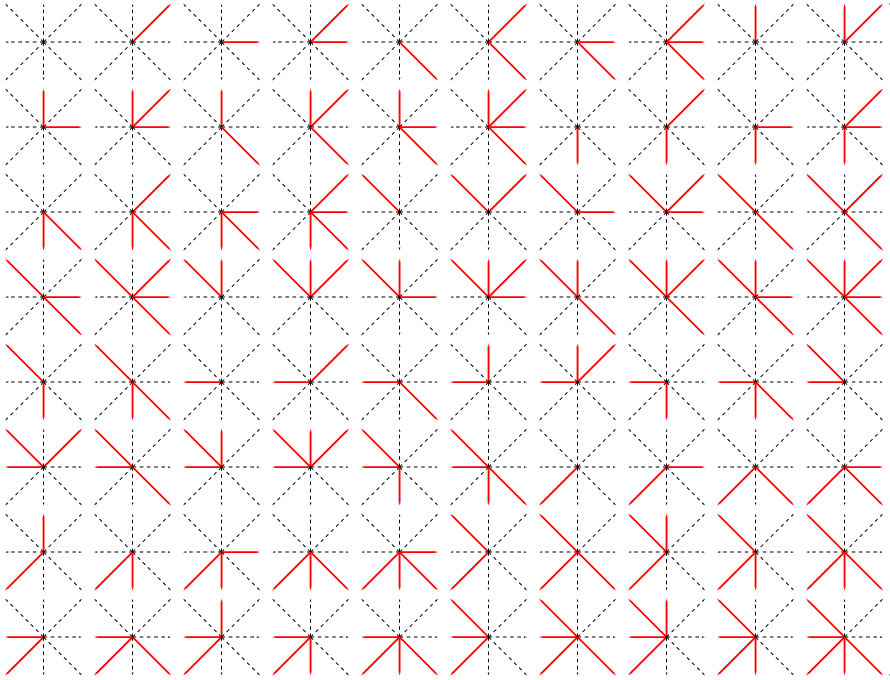
\includegraphics[scale=0.7]{TrivialWalks}

There are $2^5 = 32$ types of walks that don't leave the origin. Those are walks with steps among the set $\{$NW,W,SW,S,SE$\}$. Next we look at the walks that leave the origin but never come back.  There is the case of $S = \{NE\}$ that never comes back to any axis. Let's look at those walks that never come back to the $x_1$ axis. We have some steps that go in the positive $x_2$ direction, that is one of $\{$N, NE, E$\}$ together with some steps from $\{$NW, W, SW$\}$. If we were to include any other steps we would come back to the $x_1$ axis. If we only have a N step, we have 8 new cases, if we have only a NE step we have 3 new cases and if we have both, we have 4 new cases. This gives a total of 15 new cases. There's an equivalent number of walks that leave the $x_2$ axis and never come back to it. The running total is $32 + 1  + 15 + 15 = 63$.

To finish off we have 17 cases of walks that leave the origin, eventually interact with both axes but never come back to the origin. For this we must only include steps in such a way that we cannot pick a selection of steps that will decrease both the $x_1$ and $x_2$ coordinates. We have to pick a subset of steps from $\{$N, NE, E$\}$ so the only other steps allowed are NW and SE. The new cases coming from $\{$N, NE, E$\}$, $\{$N,E$\}$, $\{$N, NE $\}$, $\{$NE, E$\}$, $\{$N$\}$, $\{$NE$\}$, $\{$E$\}$ are 4, 4, 2, 2, 1, 2, 2 respectively.

Before we consider walks that come back to the origin we'll look at the behavior $Q$ depending on whether $S$ factors in some nice way or not.

%=======================================
\subsection{Simple case: Factoring $S$ into a product}
%=======================================

There's something we can say about the case where $S$ factors as $S = S_1(x_1)S_2(x_2)$. We have
\[
	 (DS)^k = (D_1D_2S_1S_2)^k = (D_1S_1)^k(D_2S_2)^k
\]
since the $D_1$ and $D_2$ operators commute and the $D_iS_i$ operators also commute since they deal with different variables. The functional equation for $Q$ is
\[
	(1-tDS)Q = 1
\]
We can compute $Q$ directly via the iteration as 
\[
	Q = \sum_{k = 0}^{\infty} t^k (DS)^k = \sum_{k = 0}^{\infty} t^k (D_1S_1)^k(D_2S_2)^k = Q_1(x_1, a_1,t) \odot_t Q_2(x_2,a_2,t)
\]
where $\odot_t$ denotes the Hadamard product of two functions with respect to variable $t$. From now on we'll drop the subscript $t$ unless it is needed. Here $Q_i$ is given by
\[
	Q_i = \sum_{k = 0}^{\infty} t^k (D_iS_i)^k
\]
and by reversing the iteration we obtain the functional equation
\[
	(1-tD_iS_i)Q_i = 1
\]
In other words, $Q_i(x_i,a_i,t)$ is the generating function for a 1-dimensional problem with Laurent step polynomial $S_i(x_i)$. In the case of a factoring of this sort, we are able to glue the 2-dimensional solution out of two 1-dimensional solutions. If we want to look at the generating function for quarter plane walks of length $k$ it is enough to look at the product of two generating functions for one-dimensional walks of length $k$. Also, we can write
\begin{align*}
	Q &= Q_1 \odot Q_2, \quad \wh Q = \wh Q_1 \odot Q_2\\
	\wc Q &= Q_1 \odot \wc Q_2, \quad \wc{\wh Q}  = \wh Q_1 \odot \wc Q_2
\end{align*}
Therefore
\begin{align*}
	B_1 B_2 Q = Q-\wh Q -\wc Q + \wc{\wh Q} &= (Q_1 - \wh Q_1)\odot (Q_2 - \wc Q_2) \\
	B_1B_2(Q_1\odot Q_2) &=( B_1 Q_1) \odot ( B_2 Q_2)
\end{align*}
In general if we are applying operators that don't involve $t$ to a Hadamard product with respect to $t$ we can treat the operator as a constant with respect to $t$ and apply it on whichever term we would like to. If it applies to both terms then we have to apply it to their mixture in a non-trivial way. For example, each of the $Q_i$'s solves a 1-dimensional problem and therefore we have a relationship of the type $B_i (f_i Q_i) = g_i$ for some $f_i$ and $g_i$. Then we can write
\[
	B_1 B_2 (f_1 Q_1 \odot f_2 Q_2) = ( B_1 f_1 Q_1) \odot ( B_2 f_2 Q_2) = g_1 \odot g_2
\]
but so far this is not a relationship of the type $B_1B_2 (fQ) = g$ since taking out the functions $f_1$ and $f_2$ from within the Hadamard product is non-trivial in general. One might be tempted to say that $f = f_1 \odot f_2$ but that would be incorrect. It would be neat to see if there is a way to find $f$ in terms of $f_1$ and $f_2$.

There is a way to see the Hadamard product solution without the iteration method. Suppose that $Q_i$ is a solution to the functional equation $(M_i - tE_iS_i)Q_i = \ol{a}_i$ for $i = 1$ and $i = 2$. Then we claim that $Q = Q_1 \odot Q_2$ is a solution to the functional equation $(M - tES)Q = \ol{a}_1\ol{a}_2$. To this end we calculate
\begin{align*}
	(M-tES)Q &= M (Q_1\odot Q_2) - tES(Q_1\odot Q_2)\\
	& = (M_1Q_1\odot M_2Q_2) - t((E_1S_1Q_1)\odot (E_2S_2Q_2))\\
\end{align*}
Then we substitute $ M_i Q_i = \ol{a}_i + tE_iS_iQ_i$ into the first term to obtain
\begin{align*}
	 (M_1Q_1\odot M_2Q_2) &= (\ol{a}_1+ t E_1 S_1 Q_1)\odot(\ol{a}_2 + t E_2 S_2 Q_2)\\
	 & = \ol{a}_1\odot\ol{a}_2 + \ol{a}_1\odot (t E_2 S_2 Q_2) + \ol{a}_2\odot(t E_1 S_1 Q_1) + (t E_1 S_1 Q_1)\odot(t E_2 S_2 Q_2))
\end{align*}
We have
\[
	\ol{a}_i\odot (t E_j S_j Q_j) = \ol{a}_i [t^0]t E_j S_j Q_j = 0
\]
since we are dealing with power series in $t$. Therefore
\[
	(M_1Q_1\odot M_2Q_2) =  \ol{a}_1\ol{a}_2 +t ((E_1 S_1 Q_1)\odot (E_2 S_2 Q_2))
\]
and upon substitution we are left with $\ol{a}_1\ol{a}_2$ which is what we needed in the first place.

One may also ask whether we can do something in the case where $S$ factors and the terms share variables.

This factoring also generalizes to higher dimensions. If $S$ factors into a product of $k$ factors $S_1,\ldots, S_k$ where no two of which share any variables then the problem of finding $Q$ boils down to solving $k$ lower-dimensional problems for functions $Q_1,\ldots, Q_k$, naming variables appropriately and taking the Hadamard product of the functions. That is
\[
	Q = Q_1 \odot \cdots \odot Q_k
\]
The more lower-dimensional problems that we solve, the more higher dimensional problems we can solve. Although it appears that the interesting higher dimensional problems that can be solved in this manner will have a lower and lower proportion among all higher dimensional problems.
%=======================================
\subsection{Kernel Group Considerations}
%=======================================
It is important to find more functional equations if we can. One way to do this is by applying a transformation on the pair $(x_1,x_2)$ that leaves as many parts of the functional equation as we can but still adding some information in the form of a new equation. One way to do this is to cosider mapping $x_1$ and $x_2$ to some quantities separately and then consider the full group generated by such maps. Since we usually eliminate the kernel in front of $Q$ it is useful to consider transformations that preserve the kernel.  We'll call this group $G(K)$, although it won't be the full group of rational transformations preserving the kernel. For example $(x_1,x_2) \mapsto (x_2,x_1)$ will not be in the group. Any transformation on $(x_1,x_2)$ that preserves the kernel $K = 1 -tS$ must necessarily preserve the step polynomial $S$. Here
\[
	S = \alpha \ol{x} + \beta + \gamma x
\]
where $x = x_1$ or $x_2$ and $\alpha,\beta,\gamma$ change correspondingly. We consider sending $x \mapsto X$ and solve for $X$ to determine the possible transformations we can perform. That is we have
\begin{align*}
	\alpha \ol{x} + \gamma x &=\alpha \ol{X} + \gamma X\\
	\alpha(\ol{x} - \ol{X}) &= \gamma (X-x)\\
	\alpha\frac{X-x}{Xx} &= \gamma (X-x)
\end{align*}
We have cases
\begin{itemize}
\item $\alpha = 0, \gamma = 0$. The equation is then trivially true and any transformation preserves the kernel although this is not very useful though.
\item $\alpha = 0, \gamma \neq 0$. Then $ X = x$ and only the identity transformation preserves the kernel.
\item $\alpha \neq 0, \gamma = 0$. Here $X = x$ as well.
\item $\alpha \neq 0, \gamma \neq 0$. Here we either have $X = x$ or $X\neq x$ and $X = \ol{x}\alpha/\gamma = \ol{x} S_{-1}/S_1$
\end{itemize}
In conclusion, either every transformation works and we don't have an interesting case or we have the identity transformation plus a possible second one. The last transformation creates a non-trivial group and we can have groups of various orders. Let
\[
	g_1 : x_1 \mapsto \ol{x_1}\frac{S_1^{-1}}{S_1^{1}},\quad g_2 : x_2 \mapsto \ol{x_2}\frac{S_2^{-1}}{S_2^{1}}
\]
whenever the $S$ quantities are non-zero. Note that $g_i(g_i(x_1)) = x_1$, that is they are involutions. We have three cases for each $x$
\begin{itemize}
\item 1: Any transformation can be applied
\item 2: We only have the identity transformation
\item 3: We have two transformations
 \end{itemize}
 We'll combine cases for analysis in the form "case $i.j$" to mean we have case $i$ for $x_1$ and case $j$ for $x_2$.

\begin{itemize}
\item [Case 1.1:] Here we can apply any transformation on both $x_1$ and $x_2$. From the transformation analysis this means that $S_1^{-1} = S_1^1 = S_2^{-1} = S_2^1 = 0$ and thus means that we have no steps that go away from the origin. Therefore $S = \Sf{0,0}$. Thus we have only two models - no steps or a resting step. (I should include little diagrams with arrows like before).
\item[Case 1.2]: Here any transformation applies on $x_1$, so $S_1^{-1} = S_1^1 = 0$ so the model has no steps that step away from the origin in the $x_1$-direction. Since the only transformation on $x_2$ is the identity transformation we either have $S_2^{-1} = 0$ or $S_2^1 = 0$ in which case the model consists of only an up step or a down step, together with a possible resting step. Similarly, the 2.1 case involves a single $x_1$ or $\ol{x_1}$ step with a possible resting step.
\item[Case 1.3:] (and 3.1): This case is similar to the previous one except that now we have two transformations for $x_2$ and this means $S_2^{-1}, S_2^1 \neq 0$. This means we must have either both vertical steps $x_2$ and $\ol{x}_2$ in the 1.3 case or two horizontal steps $x_1$ and $\ol{x}_1$ in the 3.1 case.
\item[Case 2.2:] In this case both transformations are the identity transformations. Therefore exactly one of $S_1^{-1}$ and $S_1^1$ is zero and exactly one of $S_2^{-1}$ and $S_2^1$ is zero. WLOG, assume that $S_1^1 \neq 0, S_2^1 \neq 0$ (the other models can be obtained by a rotation around the origing of 90, 180 and 270 degrees). The possible models are (I should include the drawings): $\{$N,E,NE$\}$, $\{$N,NE$\}$, $\{$E,NE$\}$, $\{$N,E$\}$, $\{$NE$\}$. In other words, the subsets of $\{$N,E,NE$\}$ except the ones going either only in the N direction or only in the E direction. This is a case of group $G(K)$ or order 1.
\item[Case 2.3:] In this case there is only one transformation for $x_1$ and two for $x_2$. This means $S_1^{-1} = 0$ (positive case) or $S_1^{1} = 0$ (negative case). Also $S_2^{-1}, S_2^1 \neq 0$ so there must be at least one step going in the positive $x_2$ direction and one in the negative $x_2$ direction. We have 17 cases (and another 17 including a resting step). Of course in the 3.2 case we have the meaning of $x_1$ and $x_2$ reversed.This is a case of group $G(K)$ of order 2.
\item[Case 3.3:] This is the most interesting case with two transformations for $x_1$ and $x_2$ each. This means that there must be at least one step going in a positive and one going in a negative coordinate for each of $x_1$ and $x_2$. There are a lot of such cases (in the hundreds). Previous results show that the group $G(K)$ has orders 4, 6, 8 and infinity depending on the step set in question.
 \end{itemize}

%=======================================
\section{Solving basic 2D cases}
%=======================================

%=======================================
\subsection{Cases 1.1, 1.2, 1.3}
%=======================================
A quick glance at the step models involved shows that we are dealing with essentially one-dimensional problems. This means they can be solved easily explicitly. One can also note that these models are all factorable
\[
	S(x_1,x_2) = 1\cdot S(x_2)
\]
Both $Q_1$ and $Q_2$ are functions we solved for in the one-dimensional case
\[
	Q_1(x_1,a_1,t) = \frac{1}{1-a_1 t},\quad Q_2(x_2,a_2,t) = q(x_2,a_2,t)
\]
for some solution $q$ from that section. Therefore
\[
	Q(x_1,x_2,a_1,a_2,t) = Q_1(x_1,a_1,t) \odot Q_2(x_2,a_2,t) = \frac{1}{1-a_1 t}\odot q(x_2,a_2,t) = q(x_2,a_2,a_1 t)
\]
Similarly in the 2.1, 3.1 cases
\[
	Q(x_1,x_2,a_1,a_2,t) = Q_1(x_1,a_1,t) \odot Q_2(x_2,a_2,t) =  q(x_1,a_1,t) \odot \frac{1}{1-a_2 t}= q(x_1,a_1,a_2 t)
\]
and this completes the solution. What about the relationship with the $B_1B_2$ transformation? If $f(a,t)$ is the function that goes together with $q(x,a,t)$ then the function $F(a_1,a_2,t)$ that goes together with $Q(x_1,x_2,a_1,a_2,t)$ is given by
\[
	F(a_1,a_2,t) = f(a_2,a_1 t)
\]
Then we have $B_2 (FQ) = 0$ and $B_1B_2(FQ) = 0$.

%=======================================
\subsection{Case 2.2 - group of order 1}
%=======================================
A quick glance at the step models reveals that this case is mostly trivial. We have a lot of models that never leave the origin and those have a trivial solution
\[
	Q(x_1,x_2,a_1,a_2) = \frac{1}{1-a_1a_2 \Sf{0,0} t}.
\]
We also have a lot of models that are essentially one-dimensional with a single step going along an axis and some steps going off-axis where the latter steps can never be taken by a random walk in this model. They are essentially cases already covered in the previous section. Suppose that the single step is taken in the positive $x_1$ direction. This is equivalent to the $s_{-1} = 0$ case in 1D with function
\[
	q(x,a,t) = \frac{1-s_0 t}{(1-st)(1-a s_0 t)} = \frac{1-s_0 t}{(1-x_1s_1 t)(1-a s_0 t)}
\]
Then we have
\[
	Q(x_1,x_2,a_1,a_2,t) = Q_1(x_1,a_1,t) \odot Q_2(x_2,a_2,t) =  q(x_1,a_1,t) \odot \frac{1}{1-a_2 t}= q(x_1,a_1,a_2 t)
\]
and therefore
\[
	Q(x_1,x_2,a_1,a_2,t) = \frac{1-a_2 \Sf{0,0} t}{(1-(x_1+\Sf{0,0})a_2 t)(1-a_1a_2 \Sf{0,0}t)}
\]
The interesting models in case 2.2 are those with non-negative steps that we listed. Here
\[
	S = \alpha x_1 + \beta x_2 + \gamma x_1 x_2 + \delta
\]
The functional equation and its zero extractions are
\begin{align*}
(1-tS)Q - c_1 Q_1^0- c_2 Q_2^0+ c_1c_2 Q_{1,2}^{0,0}  &= \ol{a_1a_2}\\
(1-ta_1 (\delta+\beta x_2))Q_1^0 - c_2Q_{1,2}^{0,0} &=\ol{a_2}\\
(1-ta_2 (\delta+\alpha x_1))Q_2^0 - c_1Q_{1,2}^{0,0}  &=\ol{a_1}\\
(1-a_1 a_2 t \delta)Q_{1,2}^{0,0} &= 1
\end{align*}
We solve the problem by a simple back-substitution of the variables.
\begin{align*}
\Qf{0,0} & = \frac{1}{1-a_1a_2\delta t}\\
Q_1^0 & = \frac{\ol{a}_2}{1-t a_2 S_1^0}\left(1+\frac{b_2}{1-a_1a_2 \delta t}\right) = \frac{1 -  a_1 \delta t}{(1-t a_1S_1^0)(1-a_1a_2\delta t)}\\
Q_2^0 & = \frac{\ol{a}_1}{1-t a_1 S_2^0}\left(1+\frac{b_1}{1-a_1a_2 \delta t}\right) = \frac{1 -  a_2 \delta t}{(1-t a_2S_2^0)(1-a_1a_2\delta t)}\\
Q &= \frac{1}{1-tS}(\ol{a}_1\ol{a}_2 + c_1 Q_1^0 + c_2 Q_2^0 - c_1 c_2 Q_{1,2}^{0,0})\\
&=\frac{1}{1-tS}\left (\ol{a}_1\ol{a}_2 + \frac{1}{1-ta_1a_2 \delta}\left(c_1 \frac{1 -  a_1 \delta t}{1-t a_1S_1^0} + c_2 \frac{1 -  a_2 \delta t}{1-t a_2S_1^0} - c_1 c_2 \right) \right)\\
&= \frac{1}{1-tS}\left(\ol{a}_1\ol{a}_2 + \frac{1}{1-a_1a_2\delta t}(c_1 f_1(a_1,t) + c_2 f_2(a_2,t)-c_1c_2)\right)
\end{align*}
where the last line explicitly shows that $Q$ is composed of functions that depend only on one of $a_1$, $a_2$. If we want to find a relation of the type $B(FQ) = 0$ then we must first find a suitable function $F$. First of all the $1-tS$ part doesn't play a role since it doesn't depend on $a_1$ or $a_2$. Then later the variables $c_1$ and $c_2$ will vanish when extracting the coefficients of $b_1^0$ and $b_2^0$. We'll now show that the function
\[
	F(a_1,a_2,t) = 1 - a_1 a_2 \delta t
\]
works exactly. First
\[
B((1 - a_1 a_2 \delta t)\ol{a}_1\ol{a_2}) = B(\ol{a}_1\ol{a}_2 - t \delta) = B(\ol{a}_1\ol{a}_2) - B(t \delta) = \ol{a}_1\ol{a}_2- \ol{a}_2-\ol{a}_1 + 1 = c_1 c_2
\]
Then
\[
	B(c_1 f_1+ c_2 f_2-c_1c_2) = c_1 f_1 + c_2 f_2 -c_1c_2 - c_2 f_2 - c_1 f_1 = -c_2 c_2
\]
Putting the two quantities together along with dividing by $1-tS$ shows that $B(FQ) = 0$. Of course this works for $G = \Qf{0,0}$ too.

%=======================================
\subsection{Case 2.3 - group of order 2}
%=======================================
There are two possibilities here - positive and negative. In the negative case $S_1^1 = 0$ and the steps have a non-positive $x_1$ component. Due to the fact that a lot of steps are not going to be taken by random walks in those models, all of these models reduce to the cases of $S$ consising of a rest step and maybe a single step in a positive direction. This takes care of 34 models (or 68 if we include a rest step). The interesting models are those with a positive $x_1$ component, or in other words, models where $S_1^{-1} = 0$. The calculations for these models become increasingly more complicated. The functional equation and its extracted forms read as
\begin{align*}
(1-tS)Q - c_1 Q_1^0- (c_2 -t\ol{x}_2 S_2^{-1})Q_2^0+ c_1c_2 Q_{1,2}^{0,0}  &= \ol{a_1a_2}\\
(1-ta_1 S_1^0)Q_1^0 - (c_2 - ta_1 \ol{x}_2 \Sf{0,-1})Q_{1,2}^{0,0} &=\ol{a_2}\\
(1-ta_2 S_2^0)Q_2^0 - c_1Q_{1,2}^{0,0}  - a_2 t S_2^{-1} Q_2^1&=\ol{a_1}\\
(1-a_1 a_2 t \Sf{0,0})Q_{1,2}^{0,0} - ta_1 a_2 \Sf{0,-1} \Qf{0,1} &= 1
\end{align*}
This is starting to look somewhat daunting. However, we can identify a subproblem that is essentially one-dimensional and therefore already solved. For this we look at the second and fourth equations with the substitution $a_i = a, c_i = c, x_2 = x, ta_1 = \tau, S_1^0 = T, Q_1^0 (x_2)= q(x)$. These equations become
\begin{align*}
(1-\tau T)q - (c - \tau  \ol{x} T_{-1})q_0 &=\ol{a}\\
(1-a \tau T_0)q_0 - a\tau \Sf{0,-1} q_1 &= 1
\end{align*}
where $q_0 = q(a,\tau)$. This is the one-dimensional problem again. The solution here is $q(x,a,\tau)$ so the original problem has a solution
\[
	Q_1^0(x_2) = q(x_2,a_2,a_1t),\quad Q_{1,2}^{0,0} = q_0(a_2,a_1t).
\]
The reason the method worked in this case is that we have steps that keep a random walk staying on the $x_2$ axis and steps that take it away from the $x_2$ but no steps that have it return to it. This is similar to the case where a random walk leaves the $x_2$ axis never to come back. Essentially the problem splits into a one-dimensional one regarding the $x_2$ axis and a further 2D one once we step off the axis. We re-write the functional equation as
\[
	(1-tS)Q - (c_2 -t\ol{x}_2 S_2^{-1})Q_2^0  = \ol{a}_1\phi(x_2) = \ol{a_1}(\ol{a}_2 + b_1 Q_1^0 -b_1c_2Q_{1,2}^{0,0})
\]
Here we can treat $x_2$ as a constant and solve for a one-dimensional problem with $x_1$ as a variable. We can perform the same analysis as in the the one-dimensional case except where we had $\ol{a}_1$ we would now have $\ol{a}_1 \phi(x_2)$. Therefore we can solve for $Q$ explicitly. However I haven't done this yet so I'll leave this for later. Curiously enough this analysis does not use the fact that we are dealing with a group of order 2 anymore than the one-dimensional case uses the fact that $|G(K)| = 2$ for $K = 1 - t(\ol{x}+x)$. Interestingly we can try re-doing the problem using the group structure. It would surely illustrate the methods we would use later in analysing the higher group size models. I've done it on paper and I don't think I've made any mistakes. However I don't obtain the correct answers. I suspect it's because of the following - $\sigma_1 = 1/(tS_1^1) - S_1^0/S_1^1$ which does not expand as a power series in $t$. Perhaps we just cannot plug this solution into the functional equations. Therefore one would have to resort to using the $\sigma_2$ solution without being able to use the group structure at all. I can certainly solve the problem in the above manner and use the series generated for each part of the solution to test whether the second solution really fails, and if it does test if it fails because of the $\sigma_1$ behavior.
%=======================================
\section{Solving case 3.3 - supersymmetric models of order 4}
%=======================================
When we consider the supersymmetric cases the $x$-transformations are given by
\[
\bullet : x_1 \mapsto \ol{x_1},\quad\ast: x_2 \mapsto \ol{x_2}
\]
In each case we have
\[
  K^{\bullet} = K^{\ast} = K,\quad K_2^{\bullet} = K_2,\quad K_1^{\ast} = K_1
\]
while the others change in some way. The solutions eliminating the kernel also have a nice form
\[
    \sigma_i = \frac{1-S_i^0-\sqrt{(1-S_i^0)^2-4t^2 (S_i^1)^2}}{2tS_i^1},\quad\ol{\sigma_i} = \frac{1-S_i^0+\sqrt{(1-S_i^0)^2-4t^2 (S_i^1)^2}}{2tS_i^1}
\]
because we have
\[
	\ol{\sigma}_i = \frac{S_i^1}{S_i^{-1}}conj(\sigma_i) = conj(\sigma_i) 
\]
We can take the master equation and apply $\ast$ to it
\begin{align*}
-KQ + K_1 Q_1^0 + K_2 Q_2^0 - K_{1,2}Q_{1,2}^{0,0} + \alpha = 0\\
-KQ^\ast \exx+ K_1 Q_1^{0,\ast} \exx+ K_2^\ast Q_2^0 - K_{1,2}^\ast Q_{1,2}^{0,0} + \alpha = 0
\end{align*}
From here on we will input $x_1 = \sigma_1$ to rid ourselves of the kernel $K$. There will be an overloading of notation
\begin{align*}
K_1 Q_1^0 + K_2 Q_2^0 - K_{1,2}Q_{1,2}^{0,0} + \alpha = 0\\
K_1 Q_1^{0,\ast} \exx+ K_2^\ast Q_2^0 - K_{1,2}^\ast Q_{1,2}^{0,0} + \alpha = 0
\end{align*}
We can multiply both equation by something to clear $Q_2^0$ because it involves $\sigma_1$ while the other term involves only $x_2$. We have
\begin{align*}
K_1 K_2^\ast Q_1^0 +K_2^\ast K_2 Q_2^0 - K_2^\ast K_{1,2}Q_{1,2}^{0,0} + \alpha K_2^\ast= 0\\
K_1 K_2 Q_1^{0,\ast} \exx+ K_2 K_2^\ast Q_2^0 - K_2 K_{1,2}^\ast Q_{1,2}^{0,0} + \alpha K_2 = 0
\end{align*}
We subtract these two equations to obtain
\begin{align*}
    K_1(K_2^\ast Q_1 - K_2 Q_1^\ast) - ( K_2^\ast K_{1,2}- K_2 K_{1,2}^\ast)Q_{1,2}+\alpha (K_2^\ast - K_2) &= 0\\
    K_2^\ast Q_1 - K_2 Q_1^\ast - \frac{ K_2^\ast K_{1,2}- K_2 K_{1,2}^\ast}{K_1}Q_{1,2}+\alpha \frac{K_2^\ast - K_2}{K_1} &= 0\\
\end{align*}
The differences in solutions will occur from here on out.
%=======================================
\subsection{Cartesian model: steps N, S, E, W}
%=======================================
I haven't written it all up yet but we have the solution
\[
	Q = \frac{(1-b_1b_2 G)(\alpha - \ol{b}_1 K_1 \wh{K}_1^\bullet -\ol{b}_2K_2\wc{K}_2^\ast \wc{Q})}{K - \ol{c}_1 K_1 K_1^\bullet - \ol{c}_2 K_2 K_2^\ast}
\]
%=======================================
\subsection{Diagonal model: steps NE, NW, SE, SW}
%=======================================
In this case the roots of the kernel become
\[
    \sigma_i = \frac{1-\sqrt{1-4t^2 (S_i^1)^2}}{2tS_i^1},\quad\ol{\sigma_i} = \frac{1+\sqrt{1-4t^2 (S_i^1)^2}}{2tS_i^1}
\]
with the extra property that
\[
   \sigma_1+\ol{\sigma_1} = \frac{1}{tS_1^{-1}}.
\]
First we have
\begin{align*}
K_2^\ast - K_2 
&= t(\ol{x_2}-x_2)S_2^{-1}(\sigma_1)\\
&=t(\ol{x_2}-x_2)(\ol{\sigma_1}+\sigma_1)\\
&=\frac{\ol{x_2}-x_2}{\ol{x_2}+x_2}
\end{align*}
We have
\begin{align*}
K_2^\ast K_{1,2} - K_2 K_{1,2}^\ast &= (c_2-tx_2S_2^{-1})\left(c_1c_2 - t\ol{\sigma_1}\ol{x_2}\right)-(c_2-t\ol{x_2}S_2^{-1})\left(c_1c_2 - t\ol{\sigma_1}x_2\right)\\
&=c_1c_2t(\ol{x_2}-x_2)S_2^{-1} - c_2t\ol{\sigma_1}(\ol{x_2}-x_2)\\
&=c_2t(\ol{x_2}-x_2)(c_1(\sigma_1+\ol{\sigma_1})-\ol{\sigma_1})
\end{align*}
If we let $v = \ol{x_2}+x_2$ we find
\[
  \sigma_1 = \frac{1-\sqrt{1-4t^2v^2}}{2tv},\quad \ol{\sigma_1} = \frac{1+\sqrt{1-4t^2v^2}}{2tv}
\]
We have
\begin{align*}
(c_1(\sigma_1+\ol{\sigma_1})-\ol{\sigma_1})&= \frac{c1}{tv}-\frac{1+\sqrt{1-4t^2v^2}}{2tv}\\
&=\frac{1}{\ol{x_2}+x_2}\left(-\ol{a_1}+\frac{1-\sqrt{1-4t^2v^2}}{2}\right)
\end{align*}
Also
\begin{align*}
K_1 &= c_1-tv\ol{\sigma_1} \\
&= c_1-tv\frac{1+\sqrt{1-4t^2v^2}}{2tv}\\
&=1-\ol{a_1}-\frac{1+\sqrt{1-4t^2v^2}}{2}\\
&=-\ol{a_1}+\frac{1-\sqrt{1-4t^2v^2}}{2}
\end{align*}
Thus we finally have
\begin{align*}
\frac{1}{K_1}( K_2^\ast K_{1,2}- K_2 K_{1,2}^\ast) 
&= -\frac{c_2t(\ol{x_2}-x_2)(c_1(\sigma_1+\ol{\sigma_1})-\ol{\sigma_1})}{c_1-t\ol{\sigma_1}v}\\
&= -\frac{c_2t(\ol{x_2}-x_2)(-1)}{tv}\\
&= \frac{c_2(\ol{x_2}-x_2)}{\ol{x_2}+x_2}
\end{align*}
Thus the equation will now read as
\[
   K_2^\ast Q_1 - K_2 Q_1^\ast -\frac{c_2(\ol{x_2}-x_2)}{\ol{x_2}+x_2}Q_{1,2}+\alpha\frac{\ol{x_2}-x_2}{(\ol{x_2}+x_2)K_1}= 0
\]
We just need to take care of the remaining terms. We'll do this by multiplying by $\ol{x_2}+x_2$. We have
\begin{align*}
R^\ast \exx= (\ol{x_2}+x_2) K_2^\ast &= c_2(\ol{x_2}+x_2)-x_2 = c_2\ol{x_2}-\ol{a_2}x_2\\
R = (\ol{x_2}+x_2) K_2 &= c_2(\ol{x_2}+x_2)-\ol{x_2} = c_2x_2-\ol{a_2}\ol{x_2}\\
\end{align*}
We have a couple of relations here
\begin{align*}
R^\ast - R &= v(K_2^\ast-K_2) = \ol{x_2}-x_2\\
\ol{x_2}R^\ast - x_2 R &= \ol{x_2}c_2v-1- x_2 c_2v+1 \\
& = c_2v(\ol{x_2}-x_2)
\end{align*}
The equation becomes
\[
(c_2\ol{x_2}-\ol{a_2}x_2)Q_1^0(x_2)+ (\ol{a_2}\ol{x_2}-c_2x_2) Q_1^0(\ol{x_2}) - c_2(\ol{x_2}-x_2)Q_{1,2}^{0,0}+(\ol{x_2}-x_2)\ol{K}_1\alpha = 0
\]
and it's ready for extraction. Let $\delta_0 = \ol{a_1}(\ol{x_2}-x_2)\ol{K}_1$. We re-write the equation as
\[\label{zero-order}
    R^\ast Q_1^0 -R Q_1^{0,\ast} - c_2(\ol{x_2}-x_2)\Qf{0,0} +\ol{a_2}\delta_0 = 0
\]
We'll use the master equation
\[
 (1-tS)Q - (c_1-t\ol{x_1}S_1^{-1}) Q_1^0- (c_2-t\ol{x_2}S_2^{-1}) Q_2^0+ (c_1c_2-t\ol{x_1x_2}S_{1,2}^{-1,-1})Q_{1,2}^{0,0}  = \ol{a_1a_2}
\]
to further our work here. For diagonal steps it is
\[
 (1-tS)Q - (c_1-tv\ol{x_1}) Q_1^0- (c_2-t\ol{x_2}S_2^{-1}) Q_2^0+ (c_1c_2-t\ol{x_1x_2})Q_{1,2}^{0,0}  = \ol{a_1a_2}
\]
extracting the $[x_1^0]$ coefficient yields
\[
   Q_1^0 = \ol{a_2}+c_2\Qf{0,0} + a_1tvQ_1^1
\]
We can extract higher coefficients too. Let $k\geq 1$. Then the $[x_2^k]$ coefficient is
\begin{align*}
0 &= Q_1^k-tS_{1}^{-1}Q_1^{k+1}-tS_1^{0}Q_1^k-tS_1^1Q_1^{k-1}-c_2\Qf{k,0} + t\ol{x_2}(\Sf{-1,-1}\Qf{k+1,0}+\Sf{0,-1}\Qf{k,0}+\Sf{1,-1}\Qf{k-1,0})\\
&=Q_1^k-tvQ_1^{k+1}-tvQ_1^{k-1}-c_2\Qf{k,0} + t\ol{x_2}(\Qf{k+1,0}+\Qf{k-1,0})
\end{align*}
We can re-write the last one in a form more convenient for the next few steps
\[\label{formula}
   Q_1^k = tv(Q_1^{k+1}+Q_1^{k-1}) + c_2 \Qf{k,0} - t\ol{x_2}(\Qf{k+1,0}+\Qf{k-1,0})
\]
We'll use induction to prove a nice formula but for that we'll first need to establish another base case because of this splitting of cases for the coefficient extraction. We have
\begin{align*}
   Q_1^0 &= \ol{a_2}+c_2\Qf{0,0} + a_1tvQ_1^1\\
   Q_1^{0,\ast} \exx&= \ol{a_2}+c_2\Qf{0,0} + a_1tvQ_1^{1,\ast}\\
\end{align*}
Combining them with equation (\ref{zero-order}) gives
\begin{align*}
0 &= R^\ast Q_1^0 -R Q_1^{0,\ast} - c_2(\ol{x_2}-x_2)\Qf{0,0} +\ol{a_2}\delta_0 \\
&= R^\ast ( \ol{a_2}+c_2\Qf{0,0} + a_1tvQ_1^1) -R (\ol{a_2}+c_2\Qf{0,0} + a_1tvQ_1^{1,\ast}) - c_2(\ol{x_2}-x_2)\Qf{0,0} +\ol{a_2}\delta_0\\
&=a_1tv(R^\ast Q_1^1-R Q_1^{1,\ast}) + (R^\ast-R)(\ol{a_2}+c_2\Qf{0,0}) - c_2(\ol{x_2}-x_2)\Qf{0,0} +\ol{a_2}\delta_0\\
& =a_1tv(R^\ast Q_1^1-R Q_1^{1,\ast})+\ol{a_2}(\ol{x_2}-x_2)+\ol{a_2}\delta_0\\
& =a_1tv(R^\ast Q_1^1-R Q_1^{1,\ast})+\ol{a_2}((\ol{x_2}-x_2)+\delta_0)
\end{align*}
So we can write the equation
\[
        R^\ast Q_1^1-R Q_1^{1,\ast}+\ol{a_2}\delta_1 = 0
\]
where
\[
   \delta_1 = \frac{(\ol{x_2}-x_2)+\delta_0}{a_1tv}
\]
This equation together with equation (\ref{zero-order}) form the base cases for the following lemma
\begin{lemma} Let $m\ge 0$ be an integer. Then
\begin{align}\label{coeff-eqn}
   R^\ast Q_1^m -R Q_1^{m,\ast} - c_2(\ol{x_2}-x_2)\Qf{m,0} +\ol{a_2}\delta_m = 0
\end{align}
where $\delta_m$ is not a function of $a_2$.
\end{lemma}
\begin{proof}We'll show this by induction. We have the base cases $m = 0$ and $m=1$. The latter one fits the pattern because $\Qf{1,0} = 0$ since we cannot have any walks end on coordinates $(1,0)$. Now we assume that the formula is true for all cases up to and including $m$. Then we use formula (\ref{formula})
\begin{align*}
& R^\ast Q_1^m -R Q_1^{m,\ast}\\
=&tv(R^\ast Q_1^{m+1}-R Q_1^{m+1,\ast}) + tv(R^\ast Q_1^{m-1}-R Q_1^{m-1,\ast})\\
& + c_2(R^\ast-R)\Qf{m,0}-t(\ol{x_2}R^\ast-x_2 R)(\Qf{m+1,0}+\Qf{m-1,0})\\
=& tv(R^\ast Q_1^{m+1}-R Q_1^{m+1,\ast}) + tv(c_2(\ol{x_2}-x_2)\Qf{m-1,0}-\ol{a_2}\delta_{m-1})\\
& + c_2(\ol{x_2}-x_2)\Qf{m,0}-c_2tv(\ol{x_2}-x_2)(\Qf{m+1,0}+\Qf{m-1,0})\\
=& tv(R^\ast Q_1^{m+1}-R Q_1^{m+1,\ast})+ c_2(\ol{x_2}-x_2)\Qf{m,0}-c_2tv(\ol{x_2}-x_2)\Qf{m+1,0}) - \ol{a_2}tv\delta_{m-1})\\
\end{align*}
Combining this with equation (\ref{coeff-eqn}) leads to
\begin{align*}
0 &= tv(R^\ast Q_1^{m+1}-R Q_1^{m+1,\ast})-c_2tv(\ol{x_2}-x_2)\Qf{m+1,0} - \ol{a_2}tv\delta_{m-1} +\ol{a_2}\delta_m \\
 0 & = R^\ast Q_1^{m+1}-R Q_1^{m+1,\ast}-c_2(\ol{x_2}-x_2)\Qf{m+1,0}+ \ol{a_2}\delta_{m+1}
\end{align*}
where
\[
  \delta_{m+1} =\frac{\delta_m}{tv}-\delta_{m-1}
\]
This function $\delta_{m+1}$ is also not dependent on $a_2$ and this completes the proof!
\end{proof}
There is an equivalent statement for $Q_2^n$. We can expand $R^\ast$ and $R$ to a form we can use
\[
(c_2\ol{x_2}-\ol{a_2}x_2)Q_1^m(x_2) -( c_2x_2-\ol{a_2}\ol{x_2})Q_1^m(\ol{x_2}) - c_2(\ol{x_2}-x_2)\Qf{m,0} +\ol{a_2}\delta_m = 0
\]
We start by extracting the $[x_2^1]$ coefficient
\begin{align*}
& c_2\Qf{m,2}-\ol{a_2}\Qf{m,0}-c_2\Qf{m,0} +c_2\Qf{m,0}+ [x_2^1]\ol{a_2}\delta_m = 0\\
& c_2\Qf{m,2}-\ol{a_2}\Qf{m,0}+ [x_2^1]\ol{a_2}\delta_m = 0
\end{align*}
We can also extract the $[x_2^{n+1}]$ coefficient for $n\geq 2$
\[
  c_2 Q_{1,2}^{m,n+2}-\ol{a_2}Q_{1,2}^{m,n}+[x_2^{n+1}]\ol{a_2}\delta_m= 0
\]
This formula also contains the $n = 0$ case so we treat them together. We can set $a_2 = 1$ to get
\[
    -\wc{Q}_{1,2}^{m,n}+[x_2^{n+1}]\delta_m = 0
\]
Substituting this back into the above equation gives
\[
     b_2 Q_{1,2}^{m,n+2} = Q_{1,2}^{m,n} - \wc{Q}_{1,2}^{m,n}
\]
An equivalent formula can be derived if the process is followed through the use of $x_1$ instead of $x_2$ in the analysis.
\begin{corollary} For integers $m,n \ge 0$ we have the following relations
\begin{align*}
b_1 \Qf{m+2,n} &= Q_{1,2}^{m,n}-\wh{Q}_{1,2}^{m,n}\\
b_2 \Qf{m,n+2} &= Q_{1,2}^{m,n}-\wc{Q}_{1,2}^{m,n}
\end{align*}
\end{corollary}

We can sum up those equations to obtain functional equations
\begin{corollary} For integers $m \ge 0$ we have the following relations
\begin{align*}
Q_1^m - \wh{Q}_1^m &= b_1 Q_1^{m+2}\\
\wc{Q}_1^m - \wc{\wh{Q}}_1^m &= b_1 \wc{Q}_1^{m+2}\\
x_1^2(Q_2^n-\wh{Q}_2^n) &= b_1 (Q_2^n - Q_{1,2}^{1,n}x_1 - Q_{1,2}^{0,n})\\
x_1^2(\wc{Q}_2^n-\wc{\wh{Q}}_2^n) &= b_1 (\wc{Q}_2^n - \wc{Q}_{1,2}^{1,n}x_1 - \wc{Q}_{1,2}^{0,n})\\
x_1^2(Q-\wh{Q}) &= b_1(Q-x_1Q_1^1-Q_1^0)\\
x_1^2(\wc{Q}-\wc{\wh{Q}}) &= b_1(\wc{Q}-x_1\wc{Q}_1^1-\wc{Q}_1^0)
\end{align*}
\end{corollary}

\begin{corollary} For integers $n \ge 0$ we have the following relations
\begin{align*}
Q_2^n-\wc{Q}_2^n &= b_2 Q_2^{n+2}\\
\wh{Q}_2^n-\wc{\wh{Q}}_2^n &= b_2 \wh{Q}_2^{n+2}\\
x_2^2(Q_1^m-\wc{Q}_1^m) &=  b_2 (Q_1^m - Q_{1,2}^{m,1}x_1 - Q_{1,2}^{m,0})\\
x_2^2(\wh{Q}_1^m-\wc{\wh{Q}}_1^m) &=  b_2 (\wh{Q}_1^m - \wh{Q}_{1,2}^{m,1}x_1 - \wh{Q}_{1,2}^{m,0})\\
x_2^2(Q-\wc{Q}) &= b_2(Q-x_2Q_2^1-Q_2^0)\\
x_2^2(\wh{Q}-\wc{\wh{Q}}) &= b_2(\wh{Q}-x_2\wh{Q}_2^1-\wh{Q}_2^0)
\end{align*}
\end{corollary}
Every other equation is obtained from the previous one by either setting $a_1 = 1$ or $a_2 = 1$. Here we can hope to set some telescoping sum type of thing in order to say more about $Q_{1,2}^{0,0}$

Now we can move onto the main result about the diagonal walks and it is that the function for labelled walks ending at $(0,0)$ is connected to the functions for semi-labelled and unlabelled walks endind at $(0,0)$. We can use the master equation to extract the $[x_1^0x_2^0]$ and $[x_1^1x_2^1]$ coefficients yielding the following two relations
\begin{align*}
\Qf{0,0} &= 1 + ta_1a_2 \Qf{1,1}\\
\Qf{1,1} &= t(\Qf{0,0}+\Qf{2,0}+\Qf{0,2}+\Qf{2,2})
\end{align*}
We also have
\begin{align*}
b_1b_2\Qf{2,2} &= b_1(\Qf{2,0}-\wc{Q}_{1,2}^{2,0})\\
&= b_1 \Qf{2,0} - b_1\wc{Q}_{1,2}^{2,0}\\
&= \Qf{0,0}-\wh{Q}_{1,2}^{0,0}-\wc{Q}_{1,2}^{0,0}+\wc{\wh{Q}}_{1,2}^{0,0}
\end{align*}
together with
\begin{align*}
b_1b_2\Qf{2,0} &= b_2 \Qf{0,0} - b_2 \wh{Q}_{1,2}^{0,0}\\
b_1b_2\Qf{0,2} &= b_1 \Qf{0,0} - b_1 \wc{Q}_{1,2}^{0,0}
\end{align*}
We we have
\begin{align*}
b_1b_2\Qf{1,1} &= t(b_1b_2\Qf{0,0}+b_1b_2\Qf{2,0}+b_1b_2\Qf{0,2}+b_1b_2\Qf{2,2})\\
&= t(b_1b_2\Qf{0,0}+ b_2 \Qf{0,0} - b_2 \wh{Q}_{1,2}^{0,0}+ b_1 \Qf{0,0} - b_1 \wc{Q}_{1,2}^{0,0}+\Qf{0,0}-\wh{Q}_{1,2}^{0,0}-\wc{Q}_{1,2}^{0,0}+\wc{\wh{Q}}_{1,2}^{0,0})\\
&= t((b_1b_2+b_1+b_2+1)\Qf{0,0}-(b_2+1)\wh{Q}_{1,2}^{0,0}-(b_1+1)\wc{Q}_{1,2}^{0,0}+\wc{\wh{Q}}_{1,2}^{0,0})\\
&=t(a_1a_2\Qf{0,0}-a_2\wh{Q}_{1,2}^{0,0}-a_1\wc{Q}_{1,2}^{0,0}+\wc{\wh{Q}}_{1,2}^{0,0})
\end{align*}
We can finally write
\begin{align*}
b_1b_2\Qf{0,0} &= b_1b_2 + ta_1a_2b_1b_2\Qf{1,1}\\
& =  b_1b_2 + t^2a_1a_2(a_1a_2\Qf{0,0}-a_2\wh{Q}_{1,2}^{0,0}-a_1\wc{Q}_{1,2}^{0,0}+\wc{\wh{Q}}_{1,2}^{0,0})
\end{align*}
Let $G(b_1,b_2)$ stand for $Q(0,0,b_1,b_2)$ and $G_i$ has $b_i = 0$. Then we can write it all as
\[
   b_1b_2 G = b_1b_2 + t^2a_1a_2(a_1a_2G-a_2G_1-a_1G_2+G_{1,2})
\]
or written as a linear combination
\[
   (b_1b_2-t^2a_1^2a_2^2)G+t^2a_1a_2^2G_1 + t^2a_1^2a_2G_2 - t^2a_1a_2G_{1,2} = b_1b_2
\]
We can divide out by $a_1a_2$ and obtain the equation
\[
    (c_1c_2-a_1a_2t^2)G + a_2t^2G_1+a_1t^2G_2-t^2G_{1,2}=c_1c_2
\]
from which we can read off
\[
	f(a_1,a_2,t) = c_1c_2-a_1a_2t^2
\]
and
\[
    G = \frac{(c_1c_2-t^2(a_2G_1+a_1G_2-G_{1,2})}{f(a_1,a_2,t)}
\]
together with $B(fG) = c_1c_2$
Also, we can solve for $Q_i^j$ and friends, in terms of various $[b_k^l]$ extractions, so overall it should lead to a relationship of the form $B(FQ) = 0$.
%=======================================
\subsection{The almost-full model: missing steps E and W}
%=======================================

%=======================================
\subsection{The full model: all steps available}
%=======================================

%=======================================
\subsection{Conjectured relationships depending on $\Sf{-1,-1}$}
%=======================================
As we have seen whenever $\Sf{-1,-1} = 0$, $\alpha$ and $G$ tend to go together in the equations, so in the end we have a solution that depends on $\beta(G)$ multiplied by $G_1,G_2$ and/or $G_{1,2}$. In the end this leads to a rational function solution for $G$ in terms of $G_1, G_2$ and $G_{1,2}$. It's then easy to conjecture that this happens whenever we can have such an algebraic relationship. The other part of the conjecture is that we'd have a linear relationship between $G, G_1,G_2$ and $G_{1,2}$ when $\Sf{-1,-1} \neq 0$.

%=======================================
\section{A little aside}
%=======================================

If we could prove the validity of one of the functional equations in the corollaries (5th row in each corollary) we would then be able to extract coefficients and obtain the formulas in the first corollary. However, since we have a direct proof already, this section is kind of irrelevant now. We'll just keep it for now because it has some interesting math. The steps from now on are almost exactly the same as those that you'd have to do to prove the Dyck path formula. We'll prove the last one involving a $b_1$ coefficient. First we have
\begin{align*}
   K &= 1 - tS = 1 - t(x_1+\ol{x_1})(x_2+\ol{x_2})\\
   K_1 &= c_1 - t \ol{x_1} S_1^{-1} = c_1 + \wh{K}_1\\
   K_2 &= c_2 - t \ol{x_2} S_2^{-1}\\
   K_{1,2} &= c_1c_2 - t\ol{x_1x_2} = c_1c_2+\wh{K}_{1,2}
\end{align*}
We also need the coefficient extractions
\begin{align*}[x_1^0]:&\quad Q_1^0 - c_2Q_{1,2}^{0,0}-ta_1S_1^{-1}Q_1^1 =\ol{a_2}\\
[x_1^0]: &Q_1^1-tS_1^{-1}Q_1^2-tS_1^{-1}Q_1^0+ t \ol{x_2}Q_{1,2}^{2,0}+t\ol{x_2}Q_{1,2}^{0,0} = 0\\
                &-t\ol{x_1}S_1^{-1}Q_1^2+t\ol{x_1x_2}Q_{1,2}^{2,0} = t\ol{x_1}S_1^{-1}Q_1^0-t\ol{x_1x_2}Q_{1,2}^{0,0}-\ol{x_1}Q_1^1
\end{align*}
which we'll use soon. We first start with
\begin{align*}
KQ &= K_1Q_1^0 + K_2 Q_2^0-K_{1,2}Q_{1,2}^{0,0} + \ol{a_1a_2}\\ 
      &= (c_1+\wh{K}_1)Q_1^0 + K_2 Q_2^0-(c_1c_2+\wh{K}_{1,2})Q_{1,2}^{0,0} + \ol{a_1a_2}\\
K\wh{Q} &=\wh{K}_1\wh{Q}_1^0 + K_2 \wh{Q}_2^0-\wh{K}_{1,2}\wh{Q}_{1,2}^{0,0} + \ol{a_2}
\end{align*}
Then we have
\begin{align*}
KQ-K\wh{Q} &= \wh{K}_1(Q_1^0-\wh{Q}_1^0)+\wh{K}_2(Q_2^0-\wh{Q}_2^0)-\wh{K}_{1,2}(Q_{1,2}^{0,0}-\wh{Q}_{1,2}^{0,0})+(c_1Q_1^0-c_1c_2Q_{1,2}^{0,0}+\ol{a_1a_2}-\ol{a_2})\\
                     &=\wh{K}_1(Q_1^0-\wh{Q}_1^0)+\wh{K}_2(Q_2^0-\wh{Q}_2^0)-\wh{K}_{1,2}(Q_{1,2}^{0,0}-\wh{Q}_{1,2}^{0,0}) + tb_1S_1^{-1}Q_1^1
\end{align*}
Also
\begin{align*}
 \wh{K}_1(Q_1^0-\wh{Q}_1^0) -\wh{K}_{1,2}(Q_{1,2}^{0,0}-\wh{Q}_{1,2}^{0,0})=&\wh{K}_1b_1Q_1^2-\wh{K}_{1,2}b_1Q_{1,2}^{2,0}\\
=&b_1(\wh{K}_1Q_1^2-\wh{K}_{1,2}Q_{1,2}^{0,0}\\
=&b_1(-t\ol{x_1}S_1^{-1}Q_1^2+t\ol{x_1x_2}Q_{1,2}^{2,0}) \\
=&b_1(t\ol{x_1}S_1^{-1}Q_1^0-t\ol{x_1x_2}Q_{1,2}^{0,0}-\ol{x_1}Q_1^1)
\end{align*}
Next
\begin{align*}
K_2(Q_2^0-\wh{Q}_2^0) &=(c_2 -t\ol{x_1}^2S_2^{-1})\ol{x_2}b_1(Q_2^0-Q_{1,2}^{0,0})\\ 
                                                     &=-t\ol{x_1}^2\ol{x_2}b_1S_2^{-1}(Q_2^0-Q_{1,2}^{0,0})+c_2b_1\ol{x_1}^2(Q_2^0-Q_{1,2}^{0,0})
\end{align*}
We can finally combine these expressions into
\begin{align*}
x_1^2(KQ-K\wh{Q}) = b_1x_1^2(tS_1^{-1}Q_1^1+t\ol{x_1}S_1^{-1}Q_1^0-t\ol{x_1x_2}Q_{1,2}^{0,0}-\ol{x_1}Q_1^1-t\ol{x_1}^2\ol{x_2}S_2^{-1}(Q_2^0-Q_{1,2}^{0,0})+c_2\ol{x_1}^2(Q_2^0-Q_{1,2}^{0,0}))
\end{align*}
We cancel out the $b_1$ and we have the equation
\begin{align*}
KQ-K(x_1Q_1^1+Q_1^0)) &= tx_1S_1^{-1}(x_1Q_1^1+Q_1^0) - (tx_1\ol{x_2}Q_{1,2}^{0,0}+x_1Q_1^1+t\ol{x_2}S_2^{-1}(Q_2^0-Q_{1,2}^{0,0}))-c_2(Q_2-Q_{1,2}^{0,0})
\end{align*}
Note that
\[
  K+tx_1S_1^{-1} = 1- t\ol{x_1}S_1^{-1}
\]
Once we expand the $KQ$ term on the LHS we get
\begin{align*}
&c_1Q_1^0-t\ol{x_1}S_1^{-1}Q_1^0+c_2Q_2^0-t\ol{x_2}S_1^{-1}Q_2^0+c_1c_2Q_{1,2}^{0,0}+t\ol{x_1x_2}Q_{1,2}^{0,0}+\ol{a_1a_2}\\
=&(1-t\ol{x_1}S_1^{-1})(x_1Q_1^1+Q_1^0)-x_1Q_1^1+t\ol{x_1x_2}Q_{1,2}^{0,0}-t\ol{x_2}S_2^{-1}Q_2^0+c_2(Q_2^0-Q_{1,2}^{0,0})
\end{align*}
and after careful book-keeping all the terms cancel out one by one. This completes the long-winded proof of the identity.
%=======================================

\endinput

Any text after an \endinput is ignored.
You could put scraps here or things in progress.
